\documentclass[10pt, handout]{beamer}
\usepackage{pgfpages}
\setbeameroption{show notes}

\usepackage[utf8x]{inputenc}
\usepackage[T1]{fontenc}
\usepackage{lmodern}
\usepackage{microtype}
\usepackage{xspace}
%\usepackage[binary-units=true]{siunitx}
\usepackage{graphicx}
\usepackage{hyperref}
\usepackage{todonotes}
\usepackage{epstopdf}
\usepackage{array}
\usepackage{multicol}
\usepackage{multirow}
\usepackage{tabularx} 	% tabular with automatic line-break
\newcolumntype{Y}{>{\centering\arraybackslash}X} % centered column
\usepackage{amsmath}
\usepackage{grffile} 	% better name handling with graphicx
\usepackage{currfile} 	% provides relative file inclusion for tikzscale

\usepackage[]{algorithm2e}

\usepackage{tikz}
\usepackage{pgfplots}
\usepackage{tikzscale}
\pgfplotsset{compat=newest}
\usetikzlibrary{plotmarks}
\usepackage[absolute,overlay]{textpos}

% Math symbols
\usepackage{amsmath}
\usepackage{amssymb}
\usepackage{amsthm}
\DeclareMathOperator*{\argmin}{arg\,min}
\DeclareMathOperator*{\argmax}{arg\,max}
\newcommand\norm[1]{\left\lVert#1\right\rVert}

% Sets
\newcommand{\Z}{\mathbb{Z}}
\newcommand{\R}{\mathbb{R}}
\newcommand{\Rn}{\R^n}
\newcommand{\Rnn}{\R^{n \times n}}
\newcommand{\C}{\mathbb{C}}
\newcommand{\K}{\mathbb{K}}
\newcommand{\Kn}{\K^n}
\newcommand{\Knn}{\K^{n \times n}}

\newcommand\eqdef{\triangleq}

% Vectors
\newcommand{\vct}[1]{\boldsymbol{#1}}
\newcommand{\va}{\vct{a}}
\newcommand{\vb}{\vct{b}}
\newcommand{\vc}{\vct{c}}
\newcommand{\vd}{\vct{d}}
\newcommand{\ve}{\vct{e}}
\newcommand{\vf}{\vct{f}}
\newcommand{\vg}{\vct{g}}
\newcommand{\vh}{\vct{h}}
\newcommand{\vi}{\vct{i}}
\newcommand{\vj}{\vct{j}}
\newcommand{\vk}{\vct{k}}
\newcommand{\vl}{\vct{l}}
\newcommand{\vm}{\vct{m}}
\newcommand{\vn}{\vct{n}}
\newcommand{\vo}{\vct{o}}
\newcommand{\vp}{\vct{p}}
\newcommand{\vq}{\vct{q}}
\newcommand{\vr}{\vct{r}}
\newcommand{\vs}{\vct{s}}
\newcommand{\vt}{\vct{t}}
\newcommand{\vu}{\vct{u}}
\newcommand{\vv}{\vct{v}}
\newcommand{\vw}{\vct{w}}
\newcommand{\vx}{\vct{x}}
\newcommand{\vy}{\vct{y}}
\newcommand{\vz}{\vct{z}}
% Greek letter vectors
\newcommand{\valpha}{\vct{\alpha}}
\newcommand{\vbeta}{\vct{\beta}}
\newcommand{\vepsilon}{\vct{\epsilon}}
\newcommand{\vgamma}{\vct{\gamma}}
\newcommand{\vlambda}{\vct{\lambda}}
\newcommand{\vnu}{\vct{\nu}}
\newcommand{\vphi}{\vct{\phi}}
\newcommand{\vpsi}{\vct{\psi}}
\newcommand{\vtheta}{\vct{\theta}}
\newcommand{\vxi}{\vct{\xi}}
\newcommand{\vzero}{\vct{0}}
\newcommand{\vone}{\vct{1}}
% Matrices
\newcommand{\mtx}[1]{\boldsymbol{#1}}
\newcommand{\mzero}{\mtx{0}}
\newcommand{\mA}{\mtx{A}}
\newcommand{\mB}{\mtx{B}}
\newcommand{\mC}{\mtx{C}}
\newcommand{\mD}{\mtx{D}}
\newcommand{\mE}{\mtx{E}}
\newcommand{\mF}{\mtx{F}}
\newcommand{\mG}{\mtx{G}}
\newcommand{\mH}{\mtx{H}}
\newcommand{\mI}{\mtx{I}}
\newcommand{\mJ}{\mtx{J}}
\newcommand{\mK}{\mtx{K}}
\newcommand{\mL}{\mtx{L}}
\newcommand{\mM}{\mtx{M}}
\newcommand{\mN}{\mtx{N}}
\newcommand{\mO}{\mtx{O}}
\newcommand{\mP}{\mtx{P}}
\newcommand{\mQ}{\mtx{Q}}
\newcommand{\mR}{\mtx{R}}
\newcommand{\mS}{\mtx{S}}
\newcommand{\mT}{\mtx{T}}
\newcommand{\mU}{\mtx{U}}
\newcommand{\mV}{\mtx{V}}
\newcommand{\mW}{\mtx{W}}
\newcommand{\mX}{\mtx{X}}
\newcommand{\mY}{\mtx{Y}}
\newcommand{\mZ}{\mtx{Z}}

\usepackage{comment}
\usepackage{pgfpages}
\usepackage{bm}

\usetheme[progressbar=frametitle]{metropolis}
\tikzset{font={\fontsize{10pt}{12}\selectfont}}
\usepackage{hf-tikz}
\usetikzlibrary{ 
	calc,
	arrows,
	arrows.meta,
	automata, 
	shapes, 
	snakes, 
	positioning, 
	decorations,
	decorations.text,
	fit,
	matrix,
	mindmap
	}
\tikzstyle{noeud-std}=[draw,fill=black,circle,inner sep=0pt,minimum size=7pt]
\usepackage{tkz-graph}
\usepackage{xspace}
\usepackage{amsmath}
\usepackage{mathtools}

\definecolor{green}{HTML}{14B03D}
\newcommand{\payoff}[2]{{\color{green}#1}, {\color{red}#2}}

\usepackage{ellipsis}
\def\smartphone{
\includegraphics[height=1cm]{Smartphone-icon}}
\setbeamertemplate{section in toc}[sections numbered]

\title{LINMA2345 - Game theory}
\subtitle{Repeated games}
\date{\today}
\author{Antoine Gennart\and Jonathan Sarteel\and Antoine Paris}
\institute{Ecole polytechnique de Louvain}
\titlegraphic{\hfill
\includegraphics[height=0.3cm]{logo}}

\begin{document}
\maketitle

\metroset{sectionpage=none}

\begin{frame}{Outline}
    \tableofcontents
\end{frame}

\section{Finitely Repeated Games: the Prisoner's Dilemma}
\begin{frame}{Outline}
    \tableofcontents[currentsection]
\end{frame}

\begin{frame}{What is a finitely repeated games?}
    In a \textit{finitely repeated game}, players
    \begin{itemize}
        \item play the same game for a finite number of times $K$,
        \textbf{known by the players before the game starts}, and
        \item collect their payoffs after each round (and thus observe what
        the others played).
    \end{itemize}

    \begin{figure}[!ht]
        \centering
        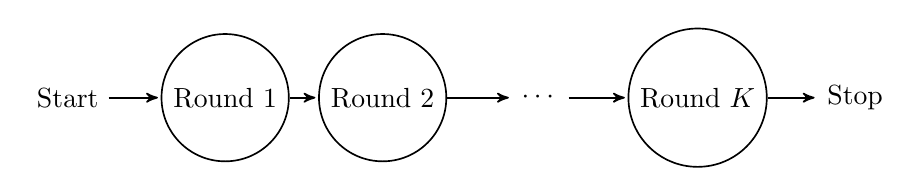
\begin{tikzpicture}[->,>=stealth',shorten >=1pt,auto,node distance=2cm, semithick, scale = 1,
            transform shape ]
            \node	        (start)								{Start};
            \node[state] 	(n1)    	[right of = start]		{Round 1};
            \node[state] 	(n2)		[right of = n1]			{Round 2};
            \node	        (dots)		[right of = n2]			{$\cdots$};
            \node[state] 	(nk)		[right of = dots]		{Round $K$};
            \node	        (stop)		[right of = nk]			{Stop};
            \path 	(start) edge node {}	(n1)
                    (n1)	edge node {}	(n2)
                    (n2)	edge node {}	(dots)
                    (dots)	edge node {}	(nk)
                    (nk) 	edge node {}	(stop);
        \end{tikzpicture}
        \caption{Finitely Repeated Games.}
    \end{figure}
\end{frame}

\begin{frame}{Let's play the Prisoner's Dilemma 2 times}
    \begin{exampleblock}{Example}
        Consider the Prisoner's Dilemma in normal form.
        \begin{table}
            \begin{tabular}{c|cc}
                & {\color{red}c}    & {\color{red}d} \\
                \hline
                {\color{green}C}    & \payoff{-1}{-1}   & \payoff{-4}{~0} \\
                {\color{green}D}    & \payoff{~0}{-4}    & \payoff{-3}{-3} 
            \end{tabular}
            \caption{Prisoner's Dilemma in normal form.}
        \end{table}
    
        \begin{itemize}
            \item The only Nash Equilibrium of this game is for both
            players to defect.
            \item Let's play this game 2 times in a row and see what happens.
        \end{itemize}
        
        \vspace{0.5cm}
        \hfill \textit{Hint}: \reflectbox{think backward}.

    \end{exampleblock}
\end{frame}

\note{
    Write the game in normal form on the blackboard as it will be used during the whole
    presentation.

    Draw a table on the blackboard and collect the actions/outcomes of each pair
    of students after each round.

    At the end, quickly compare the result. Ask students to motivate their strategy
    choice (especially if it differs from what a rational player would do).

    Probably the audience will cooperate more than expected.
}

\begin{frame}{The twice repeated Prisoner's Dilemma: Nash Equilibrium}
We proceed by \textit{backward induction} to find the Nash Equilibrium.
\begin{figure}[!ht]
    \centering
    \scalebox{0.65}{
    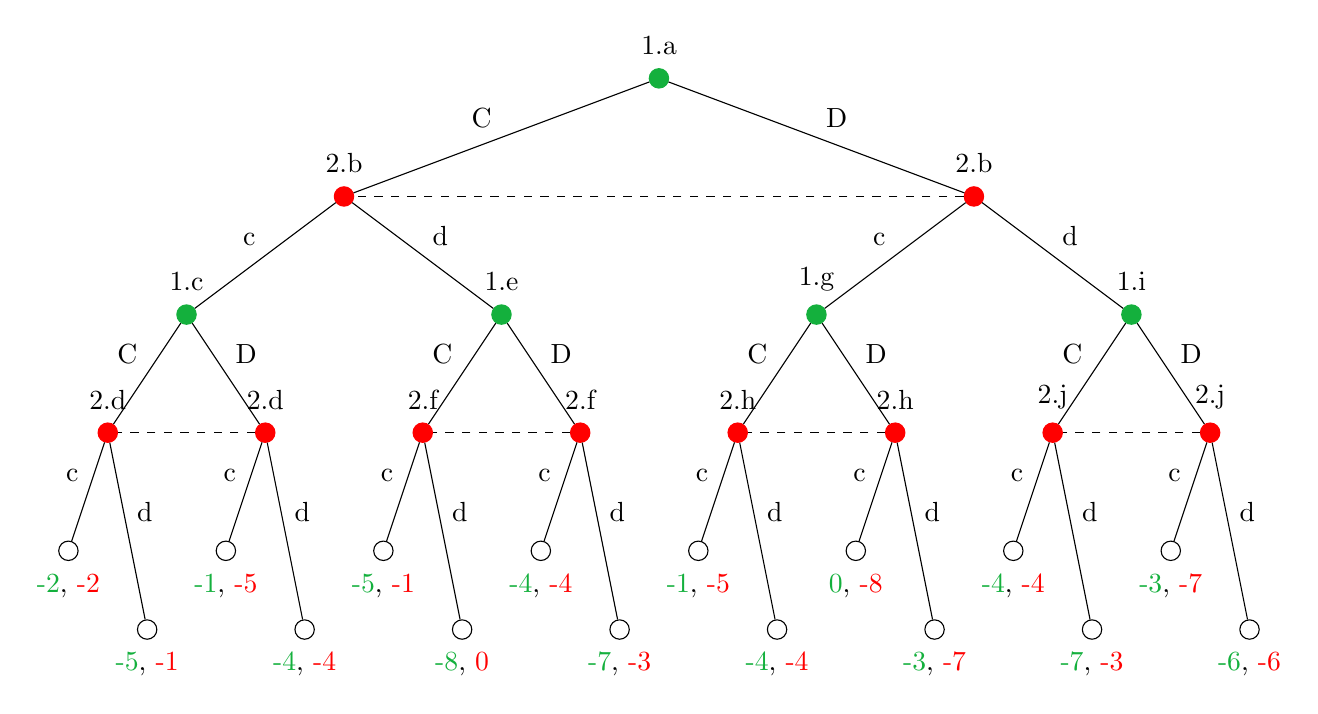
\begin{tikzpicture}
    \node[noeud-std, color=green] (n1) {}
       [sibling distance=8cm]
          child {node[noeud-std, color=red] (n2-1c) {} % 1
          [sibling distance=4cm]
                 child{node[noeud-std, color=green] (n1-1c2c){} % 2
                    [sibling distance=2cm]
                    child{node[noeud-std, color=red] (n2-1c2c1c){}  % 1
                        [sibling distance = 1cm]
                             child[level distance=1.5cm]{node[noeud-std,fill=white] (p-1c2c1c2c){} } % 1
                             child[level distance=2.5cm]{node[noeud-std,fill=white] (p-1c2c1c2d){} } % 1
                         }
                    child{node[noeud-std, color=red] (n2-1c2c1d){}  % 1
                        [sibling distance = 1cm]
                            child[level distance=1.5cm]{node[noeud-std,fill=white] (p-1c2c1d2c){} } % 1
                            child[level distance=2.5cm]{node[noeud-std,fill=white] (p-1c2c1d2d){} } % 1
                        }
                }
                child{node[noeud-std, color=green] (n1-1c2d){} % 2
                    [sibling distance=2cm]
                    child{node[noeud-std, color=red] (n2-1c2d1c){}  % 1
                        [sibling distance = 1cm]
                             child[level distance=1.5cm]{node[noeud-std,fill=white] (p-1c2d1c2c){} } % 1
                             child[level distance=2.5cm]{node[noeud-std,fill=white] (p-1c2d1c2d){} } % 1
                         }
                    child{node[noeud-std, color=red] (n2-1c2d1d){}  % 1
                        [sibling distance = 1cm]
                            child[level distance=1.5cm]{node[noeud-std,fill=white] (p-1c2d1d2c){} } % 1
                            child[level distance=2.5cm]{node[noeud-std,fill=white] (p-1c2d1d2d){} } % 1
                        }
                }
       }
       child {node[noeud-std, color=red] (n2-1d) {} % 1
          [sibling distance=4cm]
                 child{node[noeud-std, color=green] (n1-1d2c){} % 2
                    [sibling distance=2cm]
                    child{node[noeud-std, color=red] (n2-1d2c1c){}  % 1
                        [sibling distance = 1cm]
                             child[level distance=1.5cm]{node[noeud-std,fill=white] (p-1d2c1c2c){} } % 1
                             child[level distance=2.5cm]{node[noeud-std,fill=white] (p-1d2c1c2d){} } % 1
                         }
                    child{node[noeud-std, color=red] (n2-1d2c1d){}  % 1
                        [sibling distance = 1cm]
                            child[level distance=1.5cm]{node[noeud-std,fill=white] (p-1d2c1d2c){} } % 1
                            child[level distance=2.5cm]{node[noeud-std,fill=white] (p-1d2c1d2d){} } % 1
                        }
                }
                child{node[noeud-std, color=green] (n1-1d2d){} % 2
                    [sibling distance=2cm]
                    child{node[noeud-std, color=red] (n2-1d2d1c){}  % 1
                        [sibling distance = 1cm]
                             child[level distance=1.5cm]{node[noeud-std,fill=white] (p-1d2d1c2c){} } % 1
                             child[level distance=2.5cm]{node[noeud-std,fill=white] (p-1d2d1c2d){} } % 1
                         }
                    child{node[noeud-std, color=red] (n2-1d2d1d){}  % 1
                        [sibling distance = 1cm]
                            child[level distance=1.5cm]{node[noeud-std,fill=white] (p-1d2d1d2c){} } % 1
                            child[level distance=2.5cm]{node[noeud-std,fill=white] (p-1d2d1d2d){} } % 1
                        }
                }
       }

    ;
    %
    \node[above=5pt] at (n1) {1.a};
    \node[above left] at ($(n1)!{0.5}!(n2-1c)$) {C};
    \node[above right] at ($(n1)!{0.5}!(n2-1d)$) {D};

    \node[above=5pt] at (n2-1c) {2.b};
    \node[above left] at ($(n2-1c)!{0.5}!(n1-1c2c)$) {c};
    \node[above right] at ($(n2-1c)!{0.5}!(n1-1c2d)$) {d};
    \node[above=5pt] at (n1-1c2c) {1.c};
    \node[above left] at ($(n1-1c2c)!{0.5}!(n2-1c2c1c)$) {C};
    \node[above right] at ($(n1-1c2c)!{0.5}!(n2-1c2c1d)$) {D};
    \node[above=5pt] at (n2-1c2c1d) {2.d};
    \node[above left] at ($(n2-1c2c1d)!{0.5}!(p-1c2c1d2c)$) {c};
    \node[above right] at ($(n2-1c2c1d)!{0.5}!(p-1c2c1d2d)$) {d};
    \node[above=5pt] at (n2-1c2c1c) {2.d};
    \node[above left] at ($(n2-1c2c1c)!{0.5}!(p-1c2c1c2c)$) {c};
    \node[above right] at ($(n2-1c2c1c)!{0.5}!(p-1c2c1c2d)$) {d};
    \node[above=5pt] at (n1-1c2d) {1.e};
    \node[above left] at ($(n1-1c2d)!{0.5}!(n2-1c2d1c)$) {C};
    \node[above right] at ($(n1-1c2d)!{0.5}!(n2-1c2d1d)$) {D};
    \node[above=5pt] at (n2-1c2d1d) {2.f};
    \node[above left] at ($(n2-1c2d1d)!{0.5}!(p-1c2d1d2c)$) {c};
    \node[above right] at ($(n2-1c2d1d)!{0.5}!(p-1c2d1d2d)$) {d};
    \node[above=5pt] at (n2-1c2d1c) {2.f};
    \node[above left] at ($(n2-1c2d1c)!{0.5}!(p-1c2d1c2c)$) {c};
    \node[above right] at ($(n2-1c2d1c)!{0.5}!(p-1c2d1c2d)$) {d};

    \node[above=5pt] at (n2-1d) {2.b};
    \node[above left] at ($(n2-1d)!{0.5}!(n1-1d2c)$) {c};
    \node[above right] at ($(n2-1d)!{0.5}!(n1-1d2d)$) {d};
    \node[above=5pt] at (n1-1d2c) {1.g};
    \node[above left] at ($(n1-1d2c)!{0.5}!(n2-1d2c1c)$) {C};
    \node[above right] at ($(n1-1d2c)!{0.5}!(n2-1d2c1d)$) {D};
    \node[above=5pt] at (n2-1d2c1d) {2.h};
    \node[above left] at ($(n2-1d2c1d)!{0.5}!(p-1d2c1d2c)$) {c};
    \node[above right] at ($(n2-1d2c1d)!{0.5}!(p-1d2c1d2d)$) {d};
    \node[above=5pt] at (n2-1d2c1c) {2.h};
    \node[above left] at ($(n2-1d2c1c)!{0.5}!(p-1d2c1c2c)$) {c};
    \node[above right] at ($(n2-1d2c1c)!{0.5}!(p-1d2c1c2d)$) {d};
    \node[above=5pt] at (n1-1d2d) {1.i};
    \node[above left] at ($(n1-1d2d)!{0.5}!(n2-1d2d1c)$) {C};
    \node[above right] at ($(n1-1d2d)!{0.5}!(n2-1d2d1d)$) {D};
    \node[above=5pt] at (n2-1d2d1d) {2.j};
    \node[above left] at ($(n2-1d2d1d)!{0.5}!(p-1d2d1d2c)$) {c};
    \node[above right] at ($(n2-1d2d1d)!{0.5}!(p-1d2d1d2d)$) {d};
    \node[above=5pt] at (n2-1d2d1c) {2.j};
    \node[above left] at ($(n2-1d2d1c)!{0.5}!(p-1d2d1c2c)$) {c};
    \node[above right] at ($(n2-1d2d1c)!{0.5}!(p-1d2d1c2d)$) {d};

    \path (n2-1d)  edge [dashed] node {} (n2-1c);
    \path (n2-1c2c1d)  edge [dashed] node {} (n2-1c2c1c);
    \path (n2-1c2d1d)  edge [dashed] node {} (n2-1c2d1c);
    \path (n2-1d2c1d)  edge [dashed] node {} (n2-1d2c1c);
    \path (n2-1d2d1d)  edge [dashed] node {} (n2-1d2d1c);

    \node[below = 5pt] at ($(p-1c2c1c2c)$) {\payoff{-2}{-2}};
    \node[below = 5pt] at ($(p-1c2c1c2d)$) {\payoff{-5}{-1}};
    \node[below = 5pt] at ($(p-1c2c1d2c)$) {\payoff{-1}{-5}};
    \node[below = 5pt] at ($(p-1c2c1d2d)$) {\payoff{-4}{-4}};


    \node[below = 5pt] at ($(p-1c2d1c2c)$) {\payoff{-5}{-1}};
    \node[below = 5pt] at ($(p-1c2d1c2d)$) {\payoff{-8}{0}};
    \node[below = 5pt] at ($(p-1c2d1d2c)$) {\payoff{-4}{-4}};
    \node[below = 5pt] at ($(p-1c2d1d2d)$) {\payoff{-7}{-3}};


    \node[below = 5pt] at ($(p-1d2c1c2c)$) {\payoff{-1}{-5}};
    \node[below = 5pt] at ($(p-1d2c1c2d)$) {\payoff{-4}{-4}};
    \node[below = 5pt] at ($(p-1d2c1d2c)$) {\payoff{0}{-8}};
    \node[below = 5pt] at ($(p-1d2c1d2d)$) {\payoff{-3}{-7}};


    \node[below = 5pt] at ($(p-1d2d1c2c)$) {\payoff{-4}{-4}};
    \node[below = 5pt] at ($(p-1d2d1c2d)$) {\payoff{-7}{-3}};
    \node[below = 5pt] at ($(p-1d2d1d2c)$) {\payoff{-3}{-7}};
    \node[below = 5pt] at ($(p-1d2d1d2d)$) {\payoff{-6}{-6}};

    \end{tikzpicture}}
    \caption{Prisoner's Dilemma repeated twice in extensive form.}
\end{figure}

\end{frame}

\begin{frame}{Nash equilibrium: backward induction (1)}
\vspace{0.7cm}
\begin{figure}[!ht]
\centering
\scalebox{0.65}{
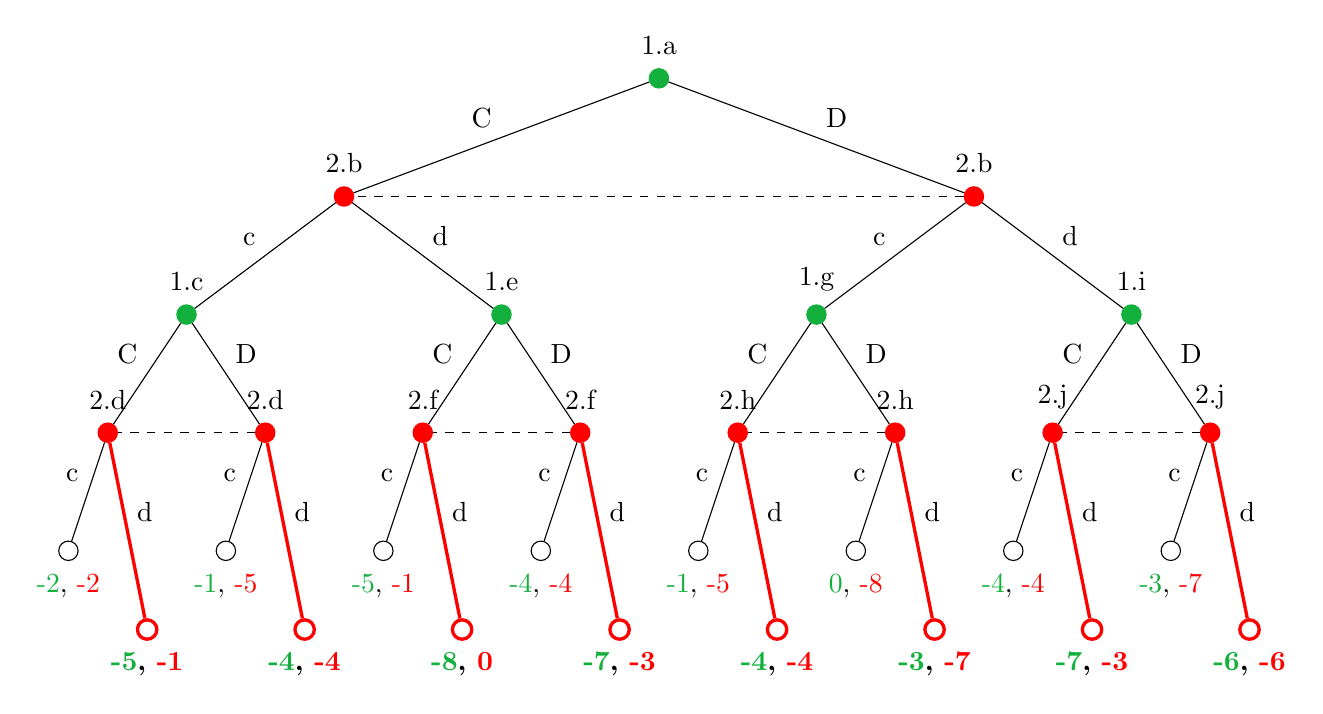
\begin{tikzpicture}
\node[noeud-std, color=green] (n1) {}
   [sibling distance=8cm]
      child {node[noeud-std, color=red] (n2-1c) {} % 1
      [sibling distance=4cm]
             child{node[noeud-std, color=green] (n1-1c2c){} % 2
                [sibling distance=2cm]
                child{node[noeud-std, color=red] (n2-1c2c1c){}  % 1
                    [sibling distance = 1cm]
                         child[level distance=1.5cm]{node[noeud-std,fill=white] (p-1c2c1c2c){} } % 1
                         child[level distance=2.5cm, very thick, red]{node[noeud-std,fill=white] (p-1c2c1c2d){} } % 1
                     }
                child{node[noeud-std, color=red] (n2-1c2c1d){}  % 1
                    [sibling distance = 1cm]
                        child[level distance=1.5cm]{node[noeud-std,fill=white] (p-1c2c1d2c){} } % 1
                        child[level distance=2.5cm, very thick, red]{node[noeud-std,fill=white] (p-1c2c1d2d){} } % 1
                    }
            }
            child{node[noeud-std, color=green] (n1-1c2d){} % 2
                [sibling distance=2cm]
                child{node[noeud-std, color=red] (n2-1c2d1c){}  % 1
                    [sibling distance = 1cm]
                         child[level distance=1.5cm]{node[noeud-std,fill=white] (p-1c2d1c2c){} } % 1
                         child[level distance=2.5cm, very thick, red]{node[noeud-std,fill=white] (p-1c2d1c2d){} } % 1
                     }
                child{node[noeud-std, color=red] (n2-1c2d1d){}  % 1
                    [sibling distance = 1cm]
                        child[level distance=1.5cm]{node[noeud-std,fill=white] (p-1c2d1d2c){} } % 1
                        child[level distance=2.5cm, very thick, red]{node[noeud-std,fill=white] (p-1c2d1d2d){} } % 1
                    }
            }
   }
   child {node[noeud-std, color=red] (n2-1d) {} % 1
      [sibling distance=4cm]
             child{node[noeud-std, color=green] (n1-1d2c){} % 2
                [sibling distance=2cm]
                child{node[noeud-std, color=red] (n2-1d2c1c){}  % 1
                    [sibling distance = 1cm]
                         child[level distance=1.5cm]{node[noeud-std,fill=white] (p-1d2c1c2c){} } % 1
                         child[level distance=2.5cm, very thick, red]{node[noeud-std,fill=white] (p-1d2c1c2d){} } % 1
                     }
                child{node[noeud-std, color=red] (n2-1d2c1d){}  % 1
                    [sibling distance = 1cm]
                        child[level distance=1.5cm]{node[noeud-std,fill=white] (p-1d2c1d2c){} } % 1
                        child[level distance=2.5cm, very thick, red]{node[noeud-std,fill=white] (p-1d2c1d2d){} } % 1
                    }
            }
            child{node[noeud-std, color=green] (n1-1d2d){} % 2
                [sibling distance=2cm]
                child{node[noeud-std, color=red] (n2-1d2d1c){}  % 1
                    [sibling distance = 1cm]
                         child[level distance=1.5cm]{node[noeud-std,fill=white] (p-1d2d1c2c){} } % 1
                         child[level distance=2.5cm, very thick, red]{node[noeud-std,fill=white] (p-1d2d1c2d){} } % 1
                     }
                child{node[noeud-std, color=red] (n2-1d2d1d){}  % 1
                    [sibling distance = 1cm]
                        child[level distance=1.5cm]{node[noeud-std,fill=white] (p-1d2d1d2c){} } % 1
                        child[level distance=2.5cm, very thick, red]{node[noeud-std,fill=white] (p-1d2d1d2d){} } % 1
                    }
            }
   }

;
%
\node[above=5pt] at (n1) {1.a};
\node[above left] at ($(n1)!{0.5}!(n2-1c)$) {C};
\node[above right] at ($(n1)!{0.5}!(n2-1d)$) {D};

\node[above=5pt] at (n2-1c) {2.b};
\node[above left] at ($(n2-1c)!{0.5}!(n1-1c2c)$) {c};
\node[above right] at ($(n2-1c)!{0.5}!(n1-1c2d)$) {d};
\node[above=5pt] at (n1-1c2c) {1.c};
\node[above left] at ($(n1-1c2c)!{0.5}!(n2-1c2c1c)$) {C};
\node[above right] at ($(n1-1c2c)!{0.5}!(n2-1c2c1d)$) {D};
\node[above=5pt] at (n2-1c2c1d) {2.d};
\node[above left] at ($(n2-1c2c1d)!{0.5}!(p-1c2c1d2c)$) {c};
\node[above right] at ($(n2-1c2c1d)!{0.5}!(p-1c2c1d2d)$) {d};
\node[above=5pt] at (n2-1c2c1c) {2.d};
\node[above left] at ($(n2-1c2c1c)!{0.5}!(p-1c2c1c2c)$) {c};
\node[above right] at ($(n2-1c2c1c)!{0.5}!(p-1c2c1c2d)$) {d};
\node[above=5pt] at (n1-1c2d) {1.e};
\node[above left] at ($(n1-1c2d)!{0.5}!(n2-1c2d1c)$) {C};
\node[above right] at ($(n1-1c2d)!{0.5}!(n2-1c2d1d)$) {D};
\node[above=5pt] at (n2-1c2d1d) {2.f};
\node[above left] at ($(n2-1c2d1d)!{0.5}!(p-1c2d1d2c)$) {c};
\node[above right] at ($(n2-1c2d1d)!{0.5}!(p-1c2d1d2d)$) {d};
\node[above=5pt] at (n2-1c2d1c) {2.f};
\node[above left] at ($(n2-1c2d1c)!{0.5}!(p-1c2d1c2c)$) {c};
\node[above right] at ($(n2-1c2d1c)!{0.5}!(p-1c2d1c2d)$) {d};

\node[above=5pt] at (n2-1d) {2.b};
\node[above left] at ($(n2-1d)!{0.5}!(n1-1d2c)$) {c};
\node[above right] at ($(n2-1d)!{0.5}!(n1-1d2d)$) {d};
\node[above=5pt] at (n1-1d2c) {1.g};
\node[above left] at ($(n1-1d2c)!{0.5}!(n2-1d2c1c)$) {C};
\node[above right] at ($(n1-1d2c)!{0.5}!(n2-1d2c1d)$) {D};
\node[above=5pt] at (n2-1d2c1d) {2.h};
\node[above left] at ($(n2-1d2c1d)!{0.5}!(p-1d2c1d2c)$) {c};
\node[above right] at ($(n2-1d2c1d)!{0.5}!(p-1d2c1d2d)$) {d};
\node[above=5pt] at (n2-1d2c1c) {2.h};
\node[above left] at ($(n2-1d2c1c)!{0.5}!(p-1d2c1c2c)$) {c};
\node[above right] at ($(n2-1d2c1c)!{0.5}!(p-1d2c1c2d)$) {d};
\node[above=5pt] at (n1-1d2d) {1.i};
\node[above left] at ($(n1-1d2d)!{0.5}!(n2-1d2d1c)$) {C};
\node[above right] at ($(n1-1d2d)!{0.5}!(n2-1d2d1d)$) {D};
\node[above=5pt] at (n2-1d2d1d) {2.j};
\node[above left] at ($(n2-1d2d1d)!{0.5}!(p-1d2d1d2c)$) {c};
\node[above right] at ($(n2-1d2d1d)!{0.5}!(p-1d2d1d2d)$) {d};
\node[above=5pt] at (n2-1d2d1c) {2.j};
\node[above left] at ($(n2-1d2d1c)!{0.5}!(p-1d2d1c2c)$) {c};
\node[above right] at ($(n2-1d2d1c)!{0.5}!(p-1d2d1c2d)$) {d};

\path (n2-1d)  edge [dashed] node {} (n2-1c);
\path (n2-1c2c1d)  edge [dashed] node {} (n2-1c2c1c);
\path (n2-1c2d1d)  edge [dashed] node {} (n2-1c2d1c);
\path (n2-1d2c1d)  edge [dashed] node {} (n2-1d2c1c);
\path (n2-1d2d1d)  edge [dashed] node {} (n2-1d2d1c);

\node[below = 5pt] at ($(p-1c2c1c2c)$) {\payoff{-2}{-2}};
\node[below = 5pt] at ($(p-1c2c1c2d)$) {\textbf{\payoff{-5}{-1}}};
\node[below = 5pt] at ($(p-1c2c1d2c)$) {\payoff{-1}{-5}};
\node[below = 5pt] at ($(p-1c2c1d2d)$) {\textbf{\payoff{-4}{-4}}};


\node[below = 5pt] at ($(p-1c2d1c2c)$) {\payoff{-5}{-1}};
\node[below = 5pt] at ($(p-1c2d1c2d)$) {\textbf{\payoff{-8}{0}}};
\node[below = 5pt] at ($(p-1c2d1d2c)$) {\payoff{-4}{-4}};
\node[below = 5pt] at ($(p-1c2d1d2d)$) {\textbf{\payoff{-7}{-3}}};


\node[below = 5pt] at ($(p-1d2c1c2c)$) {\payoff{-1}{-5}};
\node[below = 5pt] at ($(p-1d2c1c2d)$) {\textbf{\payoff{-4}{-4}}};
\node[below = 5pt] at ($(p-1d2c1d2c)$) {\payoff{0}{-8}};
\node[below = 5pt] at ($(p-1d2c1d2d)$) {\textbf{\payoff{-3}{-7}}};


\node[below = 5pt] at ($(p-1d2d1c2c)$) {\payoff{-4}{-4}};
\node[below = 5pt] at ($(p-1d2d1c2d)$) {\textbf{\payoff{-7}{-3}}};
\node[below = 5pt] at ($(p-1d2d1d2c)$) {\payoff{-3}{-7}};
\node[below = 5pt] at ($(p-1d2d1d2d)$) {\textbf{\payoff{-6}{-6}}};

\end{tikzpicture}}
\caption{Repeated Prisoner's Dilemma: backward induction step 1.}
\end{figure}

\end{frame}

\begin{frame}{Nash equilibrium: backward induction (2)}
    \begin{figure}[!ht]
    \centering
    \scalebox{0.65}{
    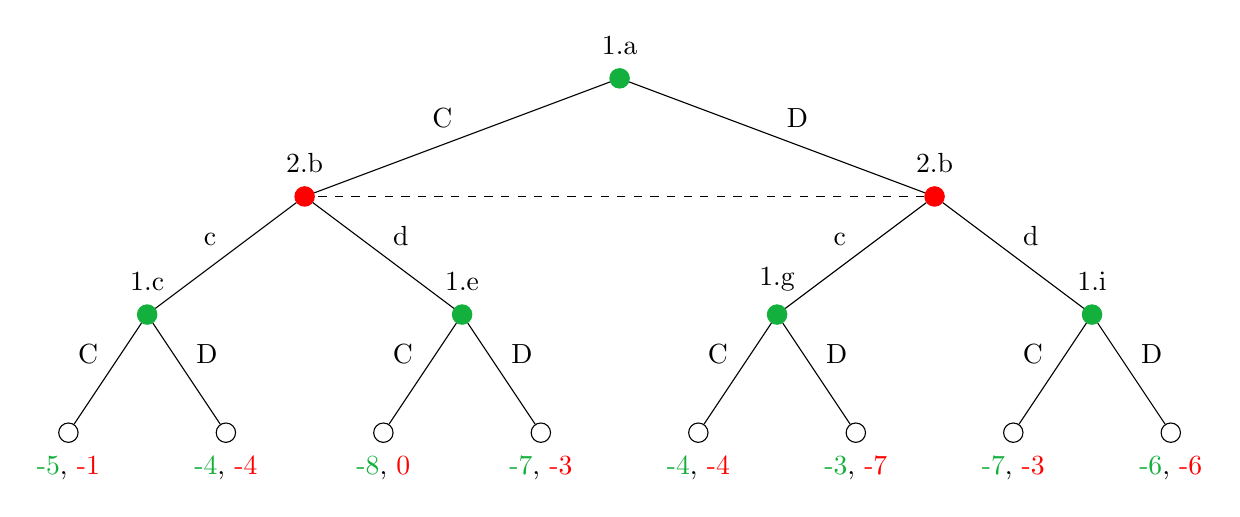
\begin{tikzpicture}
        \node[noeud-std, color=green] (n1) {}
           [sibling distance=8cm]
              child {node[noeud-std, color=red] (n2-1c) {} % 1
              [sibling distance=4cm]
                     child{node[noeud-std, color=green] (n1-1c2c){} % 2
                        [sibling distance=2cm]
                        child{node[noeud-std, fill=white] (n2-1c2c1c){}}
                        child{node[noeud-std, fill=white] (n2-1c2c1d){}}
                    }
                    child{node[noeud-std, color=green] (n1-1c2d){} % 2
                        [sibling distance=2cm]
                        child{node[noeud-std, fill=white] (n2-1c2d1c){}}
                        child{node[noeud-std, fill=white] (n2-1c2d1d){}}
                    }
           }
           child {node[noeud-std, color=red] (n2-1d) {} % 1
              [sibling distance=4cm]
                     child{node[noeud-std, color=green] (n1-1d2c){} % 2
                        [sibling distance=2cm]
                        child{node[noeud-std, fill=white] (n2-1d2c1c){}}
                        child{node[noeud-std, fill=white] (n2-1d2c1d){}}
                    }
                    child{node[noeud-std, color=green] (n1-1d2d){} % 2
                        [sibling distance=2cm]
                        child{node[noeud-std, fill=white] (n2-1d2d1c){}}
                        child{node[noeud-std, fill=white] (n2-1d2d1d){}}
                    }
           }
        ;
        %
        \node[above=5pt] at (n1) {1.a};
        \node[above left] at ($(n1)!{0.5}!(n2-1c)$) {C};
        \node[above right] at ($(n1)!{0.5}!(n2-1d)$) {D};

        \node[above=5pt] at (n2-1c) {2.b};
        \node[above left] at ($(n2-1c)!{0.5}!(n1-1c2c)$) {c};
        \node[above right] at ($(n2-1c)!{0.5}!(n1-1c2d)$) {d};
        \node[above=5pt] at (n1-1c2c) {1.c};
        \node[above left] at ($(n1-1c2c)!{0.5}!(n2-1c2c1c)$) {C};
        \node[above right] at ($(n1-1c2c)!{0.5}!(n2-1c2c1d)$) {D};
        \node[above=5pt] at (n1-1c2d) {1.e};
        \node[above left] at ($(n1-1c2d)!{0.5}!(n2-1c2d1c)$) {C};
        \node[above right] at ($(n1-1c2d)!{0.5}!(n2-1c2d1d)$) {D};

        \node[above=5pt] at (n2-1d) {2.b};
        \node[above left] at ($(n2-1d)!{0.5}!(n1-1d2c)$) {c};
        \node[above right] at ($(n2-1d)!{0.5}!(n1-1d2d)$) {d};
        \node[above=5pt] at (n1-1d2c) {1.g};
        \node[above left] at ($(n1-1d2c)!{0.5}!(n2-1d2c1c)$) {C};
        \node[above right] at ($(n1-1d2c)!{0.5}!(n2-1d2c1d)$) {D};
        \node[above=5pt] at (n1-1d2d) {1.i};
        \node[above left] at ($(n1-1d2d)!{0.5}!(n2-1d2d1c)$) {C};
        \node[above right] at ($(n1-1d2d)!{0.5}!(n2-1d2d1d)$) {D};

        \path (n2-1d)  edge [dashed] node {} (n2-1c);

        \node[below = 5pt] at ($(n2-1c2c1c)$) {\payoff{-5}{-1}};
        \node[below = 5pt] at ($(n2-1c2c1d)$) {\payoff{-4}{-4}};

        \node[below = 5pt] at ($(n2-1c2d1c)$) {\payoff{-8}{0}};
        \node[below = 5pt] at ($(n2-1c2d1d)$) {\payoff{-7}{-3}};

        \node[below = 5pt] at ($(n2-1d2c1c)$) {\payoff{-4}{-4}};
        \node[below = 5pt] at ($(n2-1d2c1d)$) {\payoff{-3}{-7}};

        \node[below = 5pt] at ($(n2-1d2d1c)$) {\payoff{-7}{-3}};
        \node[below = 5pt] at ($(n2-1d2d1d)$) {\payoff{-6}{-6}};
    \end{tikzpicture}}
    \caption{Repeated Prisoner's Dilemma: backward induction step 2.}
    \end{figure}
\end{frame}

\begin{frame}{Nash equilibrium: backward induction (3)}
    \begin{figure}[!ht]
    \centering
    \scalebox{0.65}{
    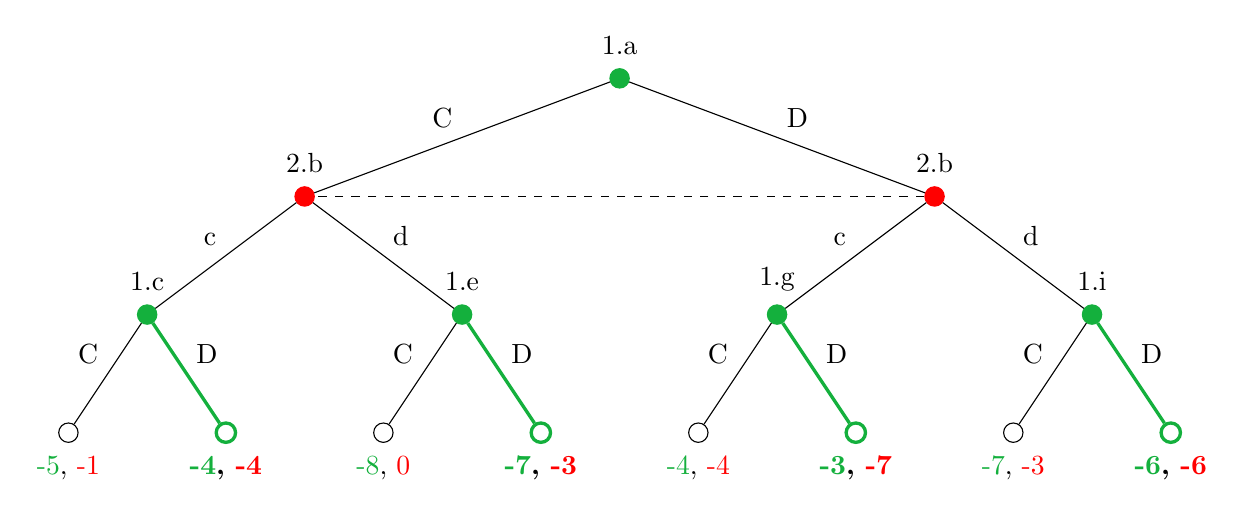
\begin{tikzpicture}
        \node[noeud-std, color=green] (n1) {}
           [sibling distance=8cm]
              child {node[noeud-std, color=red] (n2-1c) {} % 1
              [sibling distance=4cm]
                     child{node[noeud-std, color=green] (n1-1c2c){} % 2
                        [sibling distance=2cm]
                        child{node[noeud-std, fill=white] (n2-1c2c1c){}}
                        child[very thick, green]{node[noeud-std, fill=white] (n2-1c2c1d){}}
                    }
                    child{node[noeud-std, color=green] (n1-1c2d){} % 2
                        [sibling distance=2cm]
                        child{node[noeud-std, fill=white] (n2-1c2d1c){}}
                        child[very thick, green]{node[noeud-std, fill=white] (n2-1c2d1d){}}
                    }
           }
           child {node[noeud-std, color=red] (n2-1d) {} % 1
              [sibling distance=4cm]
                     child{node[noeud-std, color=green] (n1-1d2c){} % 2
                        [sibling distance=2cm]
                        child{node[noeud-std, fill=white] (n2-1d2c1c){}}
                        child[very thick, green]{node[noeud-std, fill=white] (n2-1d2c1d){}}
                    }
                    child{node[noeud-std, color=green] (n1-1d2d){} % 2
                        [sibling distance=2cm]
                        child{node[noeud-std, fill=white] (n2-1d2d1c){}}
                        child[very thick, green]{node[noeud-std, fill=white] (n2-1d2d1d){}}
                    }
           }
        ;
        %
        \node[above=5pt] at (n1) {1.a};
        \node[above left] at ($(n1)!{0.5}!(n2-1c)$) {C};
        \node[above right] at ($(n1)!{0.5}!(n2-1d)$) {D};

        \node[above=5pt] at (n2-1c) {2.b};
        \node[above left] at ($(n2-1c)!{0.5}!(n1-1c2c)$) {c};
        \node[above right] at ($(n2-1c)!{0.5}!(n1-1c2d)$) {d};
        \node[above=5pt] at (n1-1c2c) {1.c};
        \node[above left] at ($(n1-1c2c)!{0.5}!(n2-1c2c1c)$) {C};
        \node[above right] at ($(n1-1c2c)!{0.5}!(n2-1c2c1d)$) {D};
        \node[above=5pt] at (n1-1c2d) {1.e};
        \node[above left] at ($(n1-1c2d)!{0.5}!(n2-1c2d1c)$) {C};
        \node[above right] at ($(n1-1c2d)!{0.5}!(n2-1c2d1d)$) {D};

        \node[above=5pt] at (n2-1d) {2.b};
        \node[above left] at ($(n2-1d)!{0.5}!(n1-1d2c)$) {c};
        \node[above right] at ($(n2-1d)!{0.5}!(n1-1d2d)$) {d};
        \node[above=5pt] at (n1-1d2c) {1.g};
        \node[above left] at ($(n1-1d2c)!{0.5}!(n2-1d2c1c)$) {C};
        \node[above right] at ($(n1-1d2c)!{0.5}!(n2-1d2c1d)$) {D};
        \node[above=5pt] at (n1-1d2d) {1.i};
        \node[above left] at ($(n1-1d2d)!{0.5}!(n2-1d2d1c)$) {C};
        \node[above right] at ($(n1-1d2d)!{0.5}!(n2-1d2d1d)$) {D};

        \path (n2-1d)  edge [dashed] node {} (n2-1c);

        \node[below = 5pt] at ($(n2-1c2c1c)$) {\payoff{-5}{-1}};
        \node[below = 5pt] at ($(n2-1c2c1d)$) {\textbf{\payoff{-4}{-4}}};

        \node[below = 5pt] at ($(n2-1c2d1c)$) {\payoff{-8}{0}};
        \node[below = 5pt] at ($(n2-1c2d1d)$) {\textbf{\payoff{-7}{-3}}};

        \node[below = 5pt] at ($(n2-1d2c1c)$) {\payoff{-4}{-4}};
        \node[below = 5pt] at ($(n2-1d2c1d)$) {\textbf{\payoff{-3}{-7}}};

        \node[below = 5pt] at ($(n2-1d2d1c)$) {\payoff{-7}{-3}};
        \node[below = 5pt] at ($(n2-1d2d1d)$) {\textbf{\payoff{-6}{-6}}};
    \end{tikzpicture}}
    \caption{Repeated Prisoner's Dilemma: backward induction step 3.}
    \end{figure}
\end{frame}

\begin{frame}{Nash equilibrium: backward induction (4)}
    \begin{figure}[!ht]
        \centering
        \scalebox{0.65}{
        \begin{tikzpicture}
            \node[noeud-std, color=green] (n1) {}
               [sibling distance=8cm]
                  child {node[noeud-std, color=red] (n2-1c) {} % 1
                  [sibling distance=4cm]
                        child{node[noeud-std, fill=white] (n1-1c2c){}}
                        child{node[noeud-std, fill=white] (n1-1c2d){}}
               }
               child {node[noeud-std, color=red] (n2-1d) {} % 1
                  [sibling distance=4cm]
                        child{node[noeud-std, fill=white] (n1-1d2c){}}
                        child{node[noeud-std, fill=white] (n1-1d2d){}}
               }
            ;
            %
            \node[above=5pt] at (n1) {1.a};
            \node[above left] at ($(n1)!{0.5}!(n2-1c)$) {C};
            \node[above right] at ($(n1)!{0.5}!(n2-1d)$) {D};

            \node[above=5pt] at (n2-1c) {2.b};
            \node[above left] at ($(n2-1c)!{0.5}!(n1-1c2c)$) {c};
            \node[above right] at ($(n2-1c)!{0.5}!(n1-1c2d)$) {d};

            \node[above=5pt] at (n2-1d) {2.b};
            \node[above left] at ($(n2-1d)!{0.5}!(n1-1d2c)$) {c};
            \node[above right] at ($(n2-1d)!{0.5}!(n1-1d2d)$) {d};

            \path (n2-1d)  edge [dashed] node {} (n2-1c);

            \node[below = 5pt] at ($(n1-1c2c)$) {\payoff{-4}{-4}};
            \node[below = 5pt] at ($(n1-1c2d)$) {\payoff{-7}{-3}};
            \node[below = 5pt] at ($(n1-1d2c)$) {\payoff{-3}{-7}};
            \node[below = 5pt] at ($(n1-1d2d)$) {\payoff{-6}{-6}};
        \end{tikzpicture}}
        \caption{Repeated Prisoner's Dilemma: backward induction step 4.}
    \end{figure}
\end{frame}

\begin{frame}{Nash equilibrium: backward induction (5)}
    \begin{figure}[!ht]
        \centering
        \scalebox{0.65}{
        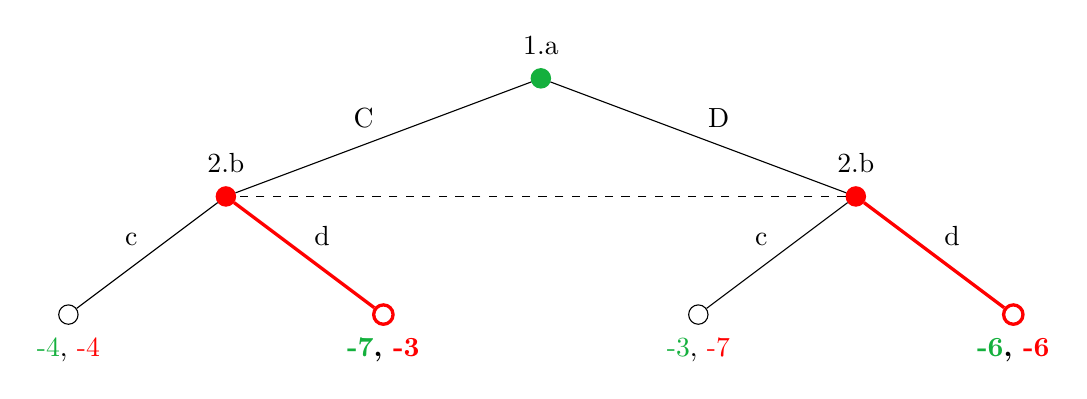
\begin{tikzpicture}
            \node[noeud-std, color=green] (n1) {}
               [sibling distance=8cm]
                  child {node[noeud-std, color=red] (n2-1c) {} % 1
                  [sibling distance=4cm]
                        child{node[noeud-std, fill=white] (n1-1c2c){}}
                        child[very thick, red]{node[noeud-std, fill=white] (n1-1c2d){}}
               }
               child {node[noeud-std, color=red] (n2-1d) {} % 1
                  [sibling distance=4cm]
                        child{node[noeud-std, fill=white] (n1-1d2c){}}
                        child[very thick, red]{node[noeud-std, fill=white] (n1-1d2d){}}
               }
            ;
            %
            \node[above=5pt] at (n1) {1.a};
            \node[above left] at ($(n1)!{0.5}!(n2-1c)$) {C};
            \node[above right] at ($(n1)!{0.5}!(n2-1d)$) {D};

            \node[above=5pt] at (n2-1c) {2.b};
            \node[above left] at ($(n2-1c)!{0.5}!(n1-1c2c)$) {c};
            \node[above right] at ($(n2-1c)!{0.5}!(n1-1c2d)$) {d};

            \node[above=5pt] at (n2-1d) {2.b};
            \node[above left] at ($(n2-1d)!{0.5}!(n1-1d2c)$) {c};
            \node[above right] at ($(n2-1d)!{0.5}!(n1-1d2d)$) {d};

            \path (n2-1d)  edge [dashed] node {} (n2-1c);

            \node[below = 5pt] at ($(n1-1c2c)$) {\payoff{-4}{-4}};
            \node[below = 5pt] at ($(n1-1c2d)$) {\textbf{\payoff{-7}{-3}}};
            \node[below = 5pt] at ($(n1-1d2c)$) {\payoff{-3}{-7}};
            \node[below = 5pt] at ($(n1-1d2d)$) {\textbf{\payoff{-6}{-6}}};
        \end{tikzpicture}}
        \caption{Repeated Prisoner's Dilemma: backward induction step 5.}
    \end{figure}
\end{frame}

\begin{frame}{Nash equilibrium: backward induction (6)}
    \begin{figure}[!ht]
        \centering
        \scalebox{0.65}{
        \begin{tikzpicture}
            \node[noeud-std, color=green] (n1) {}
                [sibling distance=8cm]
                    child {node[noeud-std, fill=white] (n2-1c) {}}
                    child {node[noeud-std, fill=white] (n2-1d) {} }
            ;
            %
            \node[above=5pt] at (n1) {1.a};
            \node[above left] at ($(n1)!{0.5}!(n2-1c)$) {C};
            \node[above right] at ($(n1)!{0.5}!(n2-1d)$) {D};

            \node[below = 5pt] at ($(n2-1c)$) {\payoff{-7}{-3}};
            \node[below = 5pt] at ($(n2-1d)$) {\payoff{-6}{-6}};
        \end{tikzpicture}}
        \caption{Repeated Prisoner's Dilemma: backward induction step 6.}
    \end{figure}
\end{frame}

\begin{frame}{Nash equilibrium: backward induction (7)}
    \begin{figure}[!ht]
        \centering
        \scalebox{0.65}{
        \begin{tikzpicture}
            \node[noeud-std, color=green] (n1) {}
                [sibling distance=8cm]
                    child {node[noeud-std, fill=white] (n2-1c) {}}
                    child[very thick, green] {node[noeud-std, fill=white] (n2-1d) {} }
            ;
            %
            \node[above=5pt] at (n1) {1.a};
            \node[above left] at ($(n1)!{0.5}!(n2-1c)$) {C};
            \node[above right] at ($(n1)!{0.5}!(n2-1d)$) {D};

            \node[below = 5pt] at ($(n2-1c)$) {\payoff{-7}{-3}};
            \node[below = 5pt] at ($(n2-1d)$) {\textbf{\payoff{-6}{-6}}};
        \end{tikzpicture}}
        \caption{Repeated Prisoner's Dilemma: backward induction step 7.}
    \end{figure}

    \begin{block}{Conclusion}
        The only Nash Equilibrium is for both players to defect at each round, leading
        to the total payoff (\payoff{-6}{-6}).
    \end{block}
\end{frame}

\begin{frame}{Take-home message \#1 and social experiments}
    \metroset{block=fill}
    \begin{block}{Take-home message \#1}
        Repeating the same game $K$ times where $K$ is known by the players before the game starts
        \textbf{do not} change the Nash equilibrium.\\\
        
        Proof? Use backward induction.
    \end{block}

    %\vspace{1cm}
    %\textbf{{\color{orange}Does this prediction match actual human behaviour?}}\\
    %No, experiments show that cooperation often appears in finitely repeated Prisoner's
    %Dilemma, contradicting backward induction\footnote{See for example
    %Matthew Embrey, Guillaume R. Fréchette, and Segvi Yuksel, \textbf{Cooperation in the
    %finitely repeated Prisoner's Dilemma}, {\color{gray}\textit{The Quarterly Journal of Economics},
    %509--511, 2018}.}.
\end{frame}

\note{
    Could be interesting to ask the audience to remember the take-home messages because
    we will randomly pick people among them at the end to check their memory.

    About the match with actual human behaviors, might be cool to reassure the audience
    on the results of their game if cooperation indeed appeared in the example.

    As an anecdote, the cited paper has "We are responsible for all errors" written in a
    footnote on the first page. I personally never saw that before.
}


\section{Infinitely Repeated Games: the Prisoner's Dilemma (again)}
\begin{frame}{Outline}
    \tableofcontents[currentsection]
\end{frame}

\begin{frame}{Let's again play the repeated Prisoner's Dilemma}
    \begin{exampleblock}{Example}
        Consider again the Prisoner's Dilemma in normal form.
        \begin{table}
            \begin{tabular}{c|cc}
                & {\color{red}c}    & {\color{red}d} \\
                \hline
                {\color{green}C}    & \payoff{-1}{-1}   & \payoff{-4}{~0} \\
                {\color{green}D}    & \payoff{~0}{-4}    & \payoff{-3}{-3} 
            \end{tabular}
            \caption{Prisoner's Dilemma in normal form.}
        \end{table}
    
        We will roll a (fair) dice after each round
        \begin{itemize}
            \item if the result is 1, the game stops,
            \item otherwise the game continues.
        \end{itemize}
        At the end of each round, you collect your payoff (and thus observe what
        the other has played).
    \end{exampleblock}
\end{frame}

\note{
    Stress that this game will be used during the whole presentation so that they should
    try to remember it.

    Ask the audience if they would change their strategy w.r.t. the previous game.
}

\begin{frame}{Can a cooperative strategy be a Nash Equilibrium?}
    \begin{block}{Cooperative strategy}
        \textit{Cooperate at each round, until the other defect,
        then defect forever} and assume both players play accordingly.
    \end{block}

    \begin{exampleblock}{For this to be a Nash Equilibrium...}
        Neither player can expect to gain by any unilateral deviation at any point
        in time (i.e., for any history of past moves).
        
        Two possible history of past moves in this case
        \begin{enumerate}
            \pause
            \item \textbf{one of the player has defected in the past}: both players are then always defecting
            and neither player could gain by deviating alone to cooperation, \pause
            \item \textbf{neither player has ever defected in the past}: both players are then always
            cooperating.
            Could it be more profitable for one player to defect? Less obvious, see blackboard!
        \end{enumerate}
    \end{exampleblock}
\end{frame}
    
\note{
    The total number of rounds follows a geometric distribution with expected value 6. That is, the
    probability that we play \textit{exactly} $k$ rounds is given by
    \[ p(k) = \left(\frac{5}{6}\right)^{k-1}\frac{1}{6}. \]

    The following formula is useful in the following reasoning
    \[ \sum_{k=1}^{\infty} kz^k = \frac{z}{(1-z)^2}. \]
}

\note{
    If both players follows the strategy and cooperate, they will each get an expected total future
    payoff of
    \begin{align*}
        \sum_{k=1}^{\infty} (-1k)\cdot p(k) &= -\frac{1}{6} \sum_{k=1}^{\infty} k\left(\frac{5}{6}\right)^{k-1}\\
                                            &= -\frac{1}{5} \sum_{k=1}^{\infty} k\left(\frac{5}{6}\right)^k \\
                                            &= -\frac{1}{5} \frac{5/6}{(1-5/6)^2} \\
                                            &= -\frac{1}{5} \frac{5}{6}\cdot 36 \\
                                            &= -6.
    \end{align*}
}

\note{
    If one of the players deviate and decide to defect, he will get 0 first and then -3 forever because the
    other player will always defect to punish him, the deviating player will then get an expected total future
    payoff of
    \begin{align*}
        0 + \sum_{k=1}^{\infty} (-3)(k-1)\cdot p(k)
        &= -\frac{1}{2} \sum_{k=2}^{\infty} (k-1)\left(\frac{5}{6}\right)^{k-1} \\
        &= -\frac{1}{2} \sum_{k'=1}^{\infty} k'\left(\frac{5}{6}\right)^{k'} \\
        &= -15 < -6.
    \end{align*}
}

\begin{frame}{Interpretation of the cooperative Nash Equilibrium}
    \begin{exampleblock}{How can we explain this cooperative equilibrium?}
        \begin{itemize}
            \item At each round, both players believe that there is a high probability that they
            will play again. The hope of \textbf{inducing a future cooperative behavior by the other
            player} can give each player an incentive to be generous.
            \item In addition, both players know that \textbf{defecting is} forever \textbf{punished} by
            the other player so that defecting, while more profitable in the short-term, is not profitable
            in the long-term.
        \end{itemize}
    \end{exampleblock}
\end{frame}

\begin{frame}{Take-home message \#2}
    \metroset{block=fill}
    \begin{block}{Take-home-message \#2}
        Rational behavior in a repeated game with a potentially infinite time horizon may be
        very different from rational behavior in the corresponding game played once (or a finite
        and known number of times).
    \end{block}
\end{frame}


\section{Infinitely Repeated Games and Utility}
\begin{frame}{Outline}
    \tableofcontents[currentsection]
\end{frame}

\begin{frame}{Infinitely Repeated Games and Utility}
    Player $i$ gets a potentially infinite sequence of payoffs
    \[ (u_i(1), u_i(2), u_i(3), \dots). \]

    \begin{alertblock}{We need a criterion for \textit{ranking} payoff sequences!}
        \pause
        \begin{itemize}
            \item Sum of payoffs as in the finitely repeated case? \textbf{No}, may be
            infinite. \pause
            \item Other criteria exist: limit of average payoff, $\delta$-discounted average,
            {\color{gray}overtaking criterion}, etc.
        \end{itemize}
    \end{alertblock}
\end{frame}

\note{
    We want to turn this infinite sequence in a single number we can reason about!

    Sum of payoffs might actually be finite in some very particular condition: there is
    an absorbing state in which the player's payoffs are always 0 and the expected number
    of rounds until arrival at this absorbing state is always finite (see Myerson).

    The overtaking criterion is in gray because it will not be covered here.
}

\begin{frame}{Limit of average payoff}
    \metroset{block=fill}
    \begin{block}{Definition}
        The limit of average of a sequence of payoffs $(u_i(1), u_i(2), u_i(3), \dots)$ is
        \[ \lim_{K\to\infty} \frac{1}{K} \sum_{k=1}^K u_i(k). \]
    \end{block}
    
    \setbeamercolor{itemize item}{fg=orange,bg=white}
    \textbf{{\color{orange}Limitations}}\\
    \pause
    \begin{itemize}
        \item The limit may not exists. \pause
        \item Let's say you play a game every year: during the first 100 years, you lose \$1M
        each year. Afterward, you win \$1 each year.\\\
            
        What is the limit of average payoffs? \pause \textbf{{\color{orange}\$1}}...
    \end{itemize}
\end{frame}

\note{
    The first limitation is mathematical and can easily be identified by the audience: we should
    ask them first.
    We should maybe also mention than there exist a way to weaken the criterion so that
    the limit always exists (using limit-infimum and limit-supremum) and redirect to Myerson
    for more details.
}

\begin{frame}{$\delta$-discounted average payoff}
    \metroset{block=fill}
    \begin{block}{Definition}
        For any \textit{discount factor} $\delta$ such that $0 \le \delta < 1$, the $\delta$-\textit{discounted
        average} of a sequence of payoffs $(u_i(1), u_i(2), u_i(3), \dots)$ is
        \[ (1-\delta)\sum_{k=1}^{\infty} \delta^{k-1}u_i(k). \]
    \end{block}

    \setbeamercolor{itemize item}{fg=green,bg=white}
    \textbf{{\color{green}Interpretations}}\\
    \pause
    \begin{itemize}
        \item The game has a probability $\delta$ of continuing at each round, the $\delta$-discounted
        average in this case is simply the expected future payoff. \pause
        \item The discount factor $\delta$ represents a \textit{measure of patience}.
    \end{itemize}
\end{frame}

\note{
    \textbf{For any general repeated game, if the payoffs are bounded, then de $\delta$-discounted
    average of each player's sequence of payoffs is a finite number and is bounded in absolute
    value by the same number that bounds payoffs}.

    Before unraveling the item in the interpretation list, we might ask if they can provided
    an interpretation based on the previous example we just saw.

    Show quickly that if $\delta = 0$, the discounted average simply give $u_i(1)$.
    While in the limit as $\delta \to 1$, the weights of each $u_i(k)$ tend to be equal.
    Important to note that this is in the limit (as for $\delta = 1$ we just get 0...).
}

\begin{frame}{Take-home message \#3}
    \metroset{block=fill}
    \begin{block}{Take-home message \#3}
        There exists several critera for ranking sequence of payoffs $(u_i(1), u_i(2), u_i(3), \dots)$
        \begin{itemize}
            \item \textit{limit of average payoffs}
            \[ \lim_{K\to\infty} \frac{1}{K} \sum_{k=1}^K u_i(k). \]
            {\color{orange}Might not exist, counter-intuitive in some case}.
            \item $\delta$\textit{-discounted average payoff}
            \[ (1-\delta)\sum_{k=1}^{\infty} \delta^{k-1}u_i(k). \]
            {\color{green}Always bounded if the payoffs are bounded, easy interpretations}. 
        \end{itemize}
    \end{block}
\end{frame}


\section{A General Model of Repeated Games}
\begin{frame}{Outline}
    \tableofcontents[currentsection]
\end{frame}

\begin{frame}{A General Model of Repeated Games}
    \tikzstyle{every picture}+=[remember picture]
    \tikzstyle{na} = [baseline=-.5ex]

    \begin{equation*}
        \Gamma^r =
            \only<1>{(
                N, \Theta, (D_i, S_i, u_i)_{i\in N}, q, p)
            }
            \only<2>{(
                \tikz[baseline]{
                    \node[fill=green!20, ellipse, anchor=base] (t1) {$N$};
                }, \Theta, (D_i, S_i, u_i)_{i\in N}, q, p)
            }
            \only<3>{(N, 
                \tikz[baseline]{
                    \node[fill=green!20, ellipse, anchor=base] (t1) {$\Theta$};
                }, (D_i, S_i, u_i)_{i\in N}, q, p)
            }
            \only<4>{(N, \Theta, (
                \tikz[baseline]{
                    \node[fill=green!20, ellipse, anchor=base] (t1) {$D_i$};
                }, S_i, u_i)_{i\in N}, q, p)
            }
            \only<5>{(N, \Theta, (D_i,
                \tikz[baseline]{
                    \node[fill=green!20, ellipse, anchor=base] (t1) {$S_i$};
                }, u_i)_{i\in N}, q, p)
            }
            \only<6>{(N, \Theta, (D_i, S_i,
                \tikz[baseline]{
                    \node[fill=green!20, ellipse, anchor=base] (t1) {$u_i$};
                })_{i\in N}, q, p)
            }
            \only<7>{(N, \Theta, (D_i, S_i, u_i)_{i\in N},
                \tikz[baseline]{
                    \node[fill=green!20, ellipse, anchor=base] (t1) {$q$};
                }, p)
            }
            \only<8>{(N, \Theta, (D_i, S_i, u_i)_{i\in N}, q,
                \tikz[baseline]{
                    \node[fill=green!20, ellipse, anchor=base] (t1) {$p$};
                })
            }
    \end{equation*}

    \begin{itemize}[<+->]
        \pause
        \item {\color<2>{green} Non-empty set of players}
        \item {\color<3>{green} Non-empty set of possible states of nature}
        \item {\color<4>{green} Set of moves player $i$ can choose at each round of the game. Let
        \[ D = \bigtimes_{i\in N} D_i .\]}
        \item {\color<5>{green} Set of signals player $i$ can receiver each round of the game. Let
        \[ S = \bigtimes_{i\in N} S_i .\]}
        \item {\color<6>{green} $u_i: D\times \Theta \to \mathbb{R}$ is the payoff function of player $i$}
        \item {\color<7>{green} $q \in \Delta(S \times \Theta)$ is the initial distribution}
        \item {\color<8>{green} $p: D\times \Theta \to \Delta(S \times \Theta)$ is the transition function}
    \end{itemize}
\end{frame}

\note{
    Model for the repeated Prisoner's Dilemma on the blackboard
    \begin{itemize}
        \item $N = \{1, 2\}$
        \item $\Theta = \{\text{active}, \text{stopped}\}$
        \item $D_1 = \{C, D\}$, $D_2 = \{c, d\}$ and $D = D_1 \times D_2$
        \item $S_i = \Theta \cup (D_1 \times D_2) = \{\text{active}, \text{stopped}, Cc, Cd, Dc, Dd\}$
        and $S = S_1 \times S_2$
        \item $u_i(d, \text{active})$ corresponds to the payoffs indicated in the normal form of the game while
        $u_i(d, \text{active}) = 0$, $\forall d \in D$
        \item $q\left((\text{active}, \text{active}), \text{active}\right) = 1$
        \item $p\left((d, d), \text{active}~|~ d, \text{active}\right) = 5/6$, 
        $p\left((\text{stopped}, \text{stopped}), \text{stopped}~|~ d, \text{active}\right)  = 1/6$ and
        $p\left((\text{stopped}, \text{stopped}), \text{stopped}~|~ d, \text{stopped}\right)  = 1$
        $\forall d \in D$
    \end{itemize}
}

\begin{frame}{Stochastic Game visualized}
    \begin{figure}
        \centering
        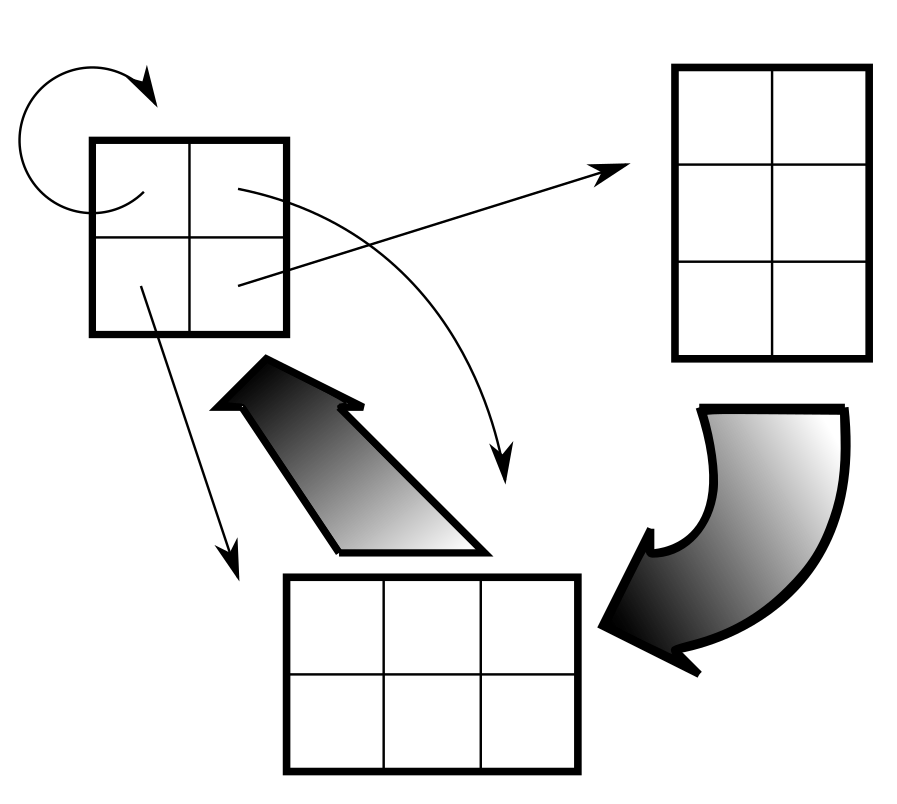
\includegraphics[width=0.6\textwidth]{img/stochastic.png}
        \caption{An illustration of what a Stochastic Game is.
        \small{Taken from ``Game Theory'' I on Coursera, by Jackson, Leyton-Brown \& Shoham.}}
    \end{figure}
\end{frame}

\note{
    \begin{itemize}
        \item agents repeatedly play games from a set of different games,
        \item the game played at each round depends on the previous game played and the
        actions taken by each players in that game.
    \end{itemize}
}

\begin{frame}{Pure strategies in infinitely repeated games}
    \begin{block}{How do we define pure strategies from that model?}
        \begin{itemize}[<+->]
            \item In a general repeated game, we assume that each player at each round $k$ recalls
            all the signals that he has gotten in rounds 1 through $k$.
            \item The set of all possible such \textit{histories of signals} for player $i$ is given by the
            $k$-fold Cartesian product of $S_i$
            \[ (S_i)^k = \underbrace{S_i \times \dots \times S_i}_{k\text{ times}}.\]
            \item A pure strategy for round $k$ is a map between each possible history in $(S_i)^k$
            and a move in $D_i$
            \[ c^k_i: (S_i)^k \to D_i. \]
            \item The set of all pure strategies for player $i$ is
            \[ C_i = \{c_i = (c_i^k)_{k=1}^\infty~|~ c_i^k: (S_i)^k \to D_i \}. \]
        \end{itemize}
    \end{block}
\end{frame}

\begin{frame}{Behavioral strategies in infinitely repeated games}
    \begin{block}{And for behavioral strategies?}
        In the same manner, the set of all behavioral strategies for player $i$ is
        \[ B_i = \{\sigma_i = (\sigma_i^k)_{k=1}^\infty~|~ \sigma_i^k: (S_i)^k
        \to {\color{green}\Delta}(D_i) \}. \]
    \end{block}
\end{frame}

\begin{frame}{Equilibrium}
    \begin{block}{Equilibrium}
        By defining some additionial quantities and doing some more {\color{orange}cumbersome}
        math, we can define what an \textit{equilibrium} is (for the different criteria for
        ranking payoffs given in the previous section).
    \end{block}

    \begin{alertblock}{Challenges}
        Because the set of behavioral strategies is \textbf{infinite}, checking if a strategy is an
        equilibrium is very hard.
    \end{alertblock}
\end{frame}

\note{
    We should briefly explain why the set of behavioral strategy is infinite here.
}

\begin{frame}{The bounded rationality principle to the rescue}
    \begin{exampleblock}{The bounded rationality principle}
        In practice, we can limit the history of past signals received to the $l$ last signals
        to define strategies.\\
        {\color{green}$\to$ the set of behavioral strategies is now finite!}
    \end{exampleblock}

    \vspace{0.5cm}
    \begin{block}{One possible interpretation}
        We can think of that as a rational players programming a computer with limited memory and
        computational power to choose its moves.
    \end{block}
\end{frame}

\begin{frame}{A Taxonomy of Repeated Games Models}
    \begin{figure}
        \tikzstyle{mybox} = [draw=gray!20, fill=white, very thick,
        rectangle, rounded corners, inner sep=10pt, inner ysep=10pt]
        \tikzstyle{fancytitle} = [fill=gray, text=white, rounded corners]
        \scalebox{0.7}{
        \begin{tikzpicture}
            \node [mybox, draw=black] at (0, 0) (gen-mod){%
                \begin{minipage}{0.50\textwidth}
                    \vspace{-0.25cm}
                    \[ \Gamma^r = (N, \Theta, (D_i, S_i, u_i)_{i\in N}, q, p) \]
                \end{minipage}
            };
            \node [inner sep=0pt] (gen-mod-img) at (-4.4, 0.5){%
                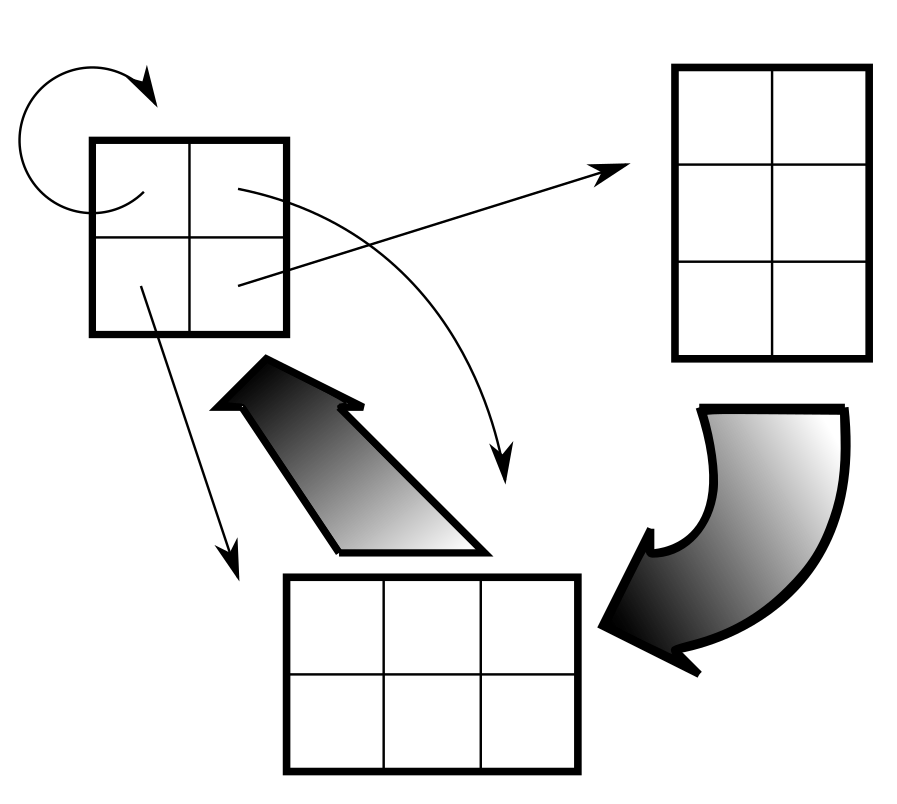
\includegraphics[width=0.25\textwidth]{img/stochastic.png}
            };
            
            \node [mybox] at (-4.5, -3) (mdp){%
                \begin{minipage}{0.40\textwidth}
                    {\color{green}Single-agent stochastic game}
                    \vspace{-0.25cm}
                    \[ |N| = 1. \]
                \end{minipage}
            };
            
            \node [mybox] at (0, -7.5) (state){%
                \begin{minipage}{\textwidth}
                    {\color{green}At every round, every player knows the
                    current state of nature $\theta \in \Theta$.} \\
                    Informally, for each player $i \in N$, there exists some
                    state $w(s_i) \in \Theta$ such that the signal $s_i$ can
                    never occur unless the current state is $w(s_i)$.
                \end{minipage}
            };
            
            \node [mybox] at (4.5, -3.5) (std){%
                \begin{minipage}{0.60\textwidth}
                    \begin{itemize}
                        \item {\color{green}Only one possible state of
                        nature}
                        \[ |\Theta| = 1. \]
                        \item {\color{green}Players know all of each other's past
                        moves}
                        \[ S_i = \bigtimes_{j\in N-i} D_j. \]
                    \end{itemize}
                \end{minipage}
            };
            \node [inner sep=0pt] (gen-mod-img) at (7, -5.5){%
                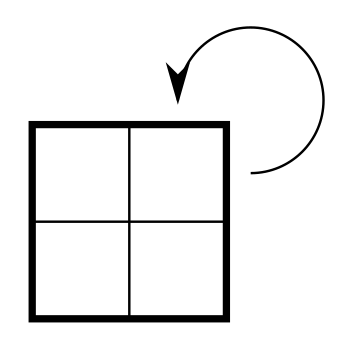
\includegraphics[width=0.20\textwidth]{img/std.png}
            };

            \node[fancytitle, fill=black] at (gen-mod.north) {Stochastic Games (General Model)};
            \node[fancytitle] at (mdp.north) (mdp-title) {Markov Decision Processes};
            \node[fancytitle] at (state.north) (state-title) {Complete State Information};
            \node[fancytitle] at (std.north) (std-title) {Standard Repeated Games};

            \draw[thick, -Latex] (gen-mod.west) -- (mdp-title.north);
            \draw[thick, -Latex] (gen-mod.south) -- (state-title.north);
            \draw[thick, -Latex] (gen-mod.east) -- (std-title.north);
        \end{tikzpicture}}
        \caption{A taxonomy of repeated game models.}
    \end{figure}
\end{frame}

\note{
    The model we just derived is the one highlighted in black.

    Explain that it generalizes Markov Decision Processes (MDPs).

    Recall the plan for the rest of the presentation by showing the two other
    models on this diagram.
}

\begin{frame}{Take-home message \#4}
    \metroset{block=fill}

    \begin{block}{Take-home message \#4}
        \begin{columns}
            \begin{column}{0.55\textwidth}
                \begin{itemize}
                    \item Stochastic Game is \textbf{the most general model} of
                    repeated games.
                    \item Generalization of \textit{Markov Decision Processes}
                    to multiple agents.
                    \item {\color{orange}The number of behavioural strategies is infinite}...
                    \item The bounded rationallity principle limits the memory (hence
                    the rationallity) of the players
                    $\to$ {\color{green}the number of behavioural strategies is finite}
                \end{itemize}
            \end{column}
            \begin{column}{0.3\textwidth}
                \begin{center}
                    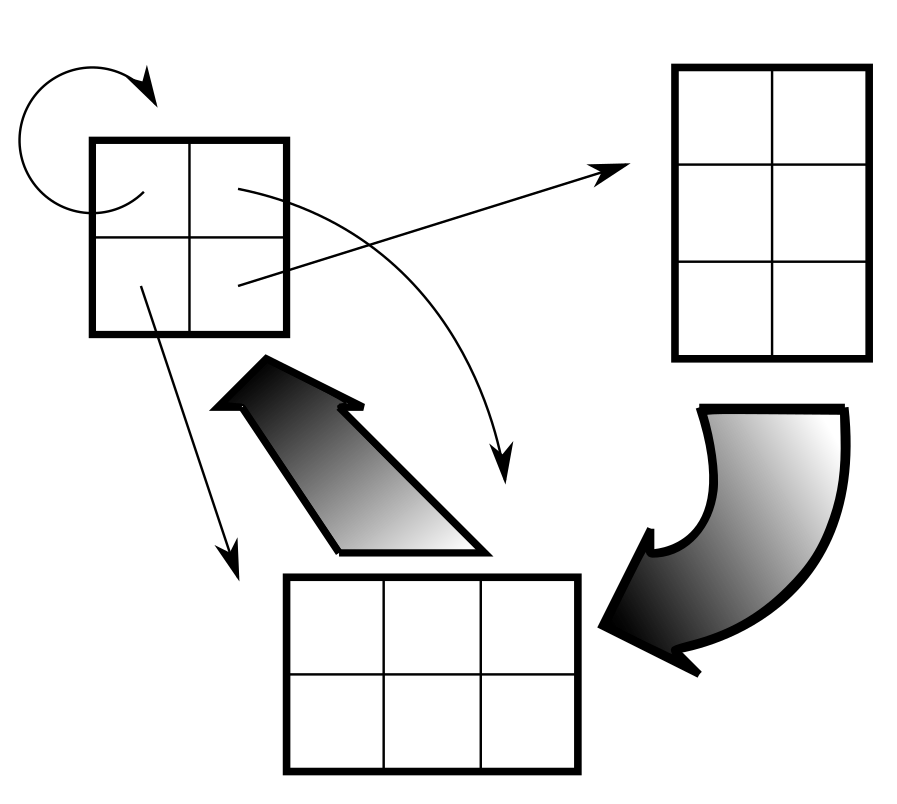
\includegraphics[width=\textwidth]{img/stochastic.png}
                    \scriptsize{\[ \Gamma^r(N, \Theta, (D_i, S_i, u_i)_{i \in N}, q, p) \]}
                \end{center}
            \end{column}
        \end{columns}

    \end{block}
\end{frame}


\section{Repeated Games with Complete State information}
\begin{frame}{Outline}
    \tableofcontents[currentsection]
\end{frame}

\section{Repeated game with complate state information}

\begin{frame}{Definition}

\textbf{Definition: }A repeated game $\Gamma^r = (N,\Theta, (D_i,S_i,u_i)_{i\in N},q,p)$ has \textit{complete state information} if, at every round, every player knows the current state of nature. That is, there is a function $\omega_i:S_i \rightarrow \Theta$ know by each player such that:
\begin{equation*}
	\forall s \in S, \forall \theta, \hat{\theta} \in \Theta, \forall d \in D : p(s,\hat{\theta} | d,\theta) = 0 \text{if} \hat{\theta} \neq \omega_i(s_i)
\end{equation*}
So the signal $s_i$ can never occur unless the current state is $\omega(s_i)$

\pause

\textbf{Definition: }In a repeated game, a game is said to be \textit{stationnary} iff the move probabiliy depends only on the current state. That is there is a function $\tau_i : \Theta \rightarrow \Delta(D_i)$ such that:
\begin{equation*}
	\forall k, \forall s \in (S)^{\times k} : \sigma_i^{[k]}(\cdot | s) = \tau_i(\cdot | \omega_i(s_i^{[k]}))
\end{equation*}
\end{frame}

\begin{frame}{Classical strategies}
\begin{itemize}
	\item \textbf{Tit-for-tat:} We begin by cooperating and then, at every round, we chose the move of our opponent at the last round.
	\item \textbf{Grim:} We begin the game with cooperation and continue cooperating at each round unless the other player defects. From this point on, we defect.
	\item \textbf{Getting-even:} We begin by cooperating, and continue cooperating unless the opponent has defected more time that we did defect. If this is the case, we defect.
\end{itemize}
\end{frame}

\begin{frame}{Small example to understand complete state information}
\textit{Consider the prisoner's dilema game in a setting where player make decision based only on the last move of they adversary.} \note{This is contrary to decision theory to make this assumption. Some strategies can still be analysed in that setting. (tit-for-tat)}

\pause
$\Rightarrow$ 4 differents states : $\Theta = \{([C,c]), ([C,d]), ([D,c]), ([D,d])\}$

\pause
If both player play the \textbf{tit-for-tat} strategy

\begin{minipage}{0.6\linewidth}
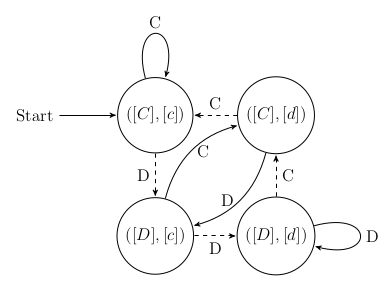
\includegraphics[width=0.9\linewidth]{img/titfortat.png}
\end{minipage}
\begin{minipage}{0.35\linewidth}
	\begin{itemize}
		\item Plain arrow if player 1 play tit-for-tat.
		\item Dashed arrow if player 1 play the opposite.
		\item Player 2 play tit-for-tat
	\end{itemize}
	\note{
		Make the graph on board if we play grim strategy
		
		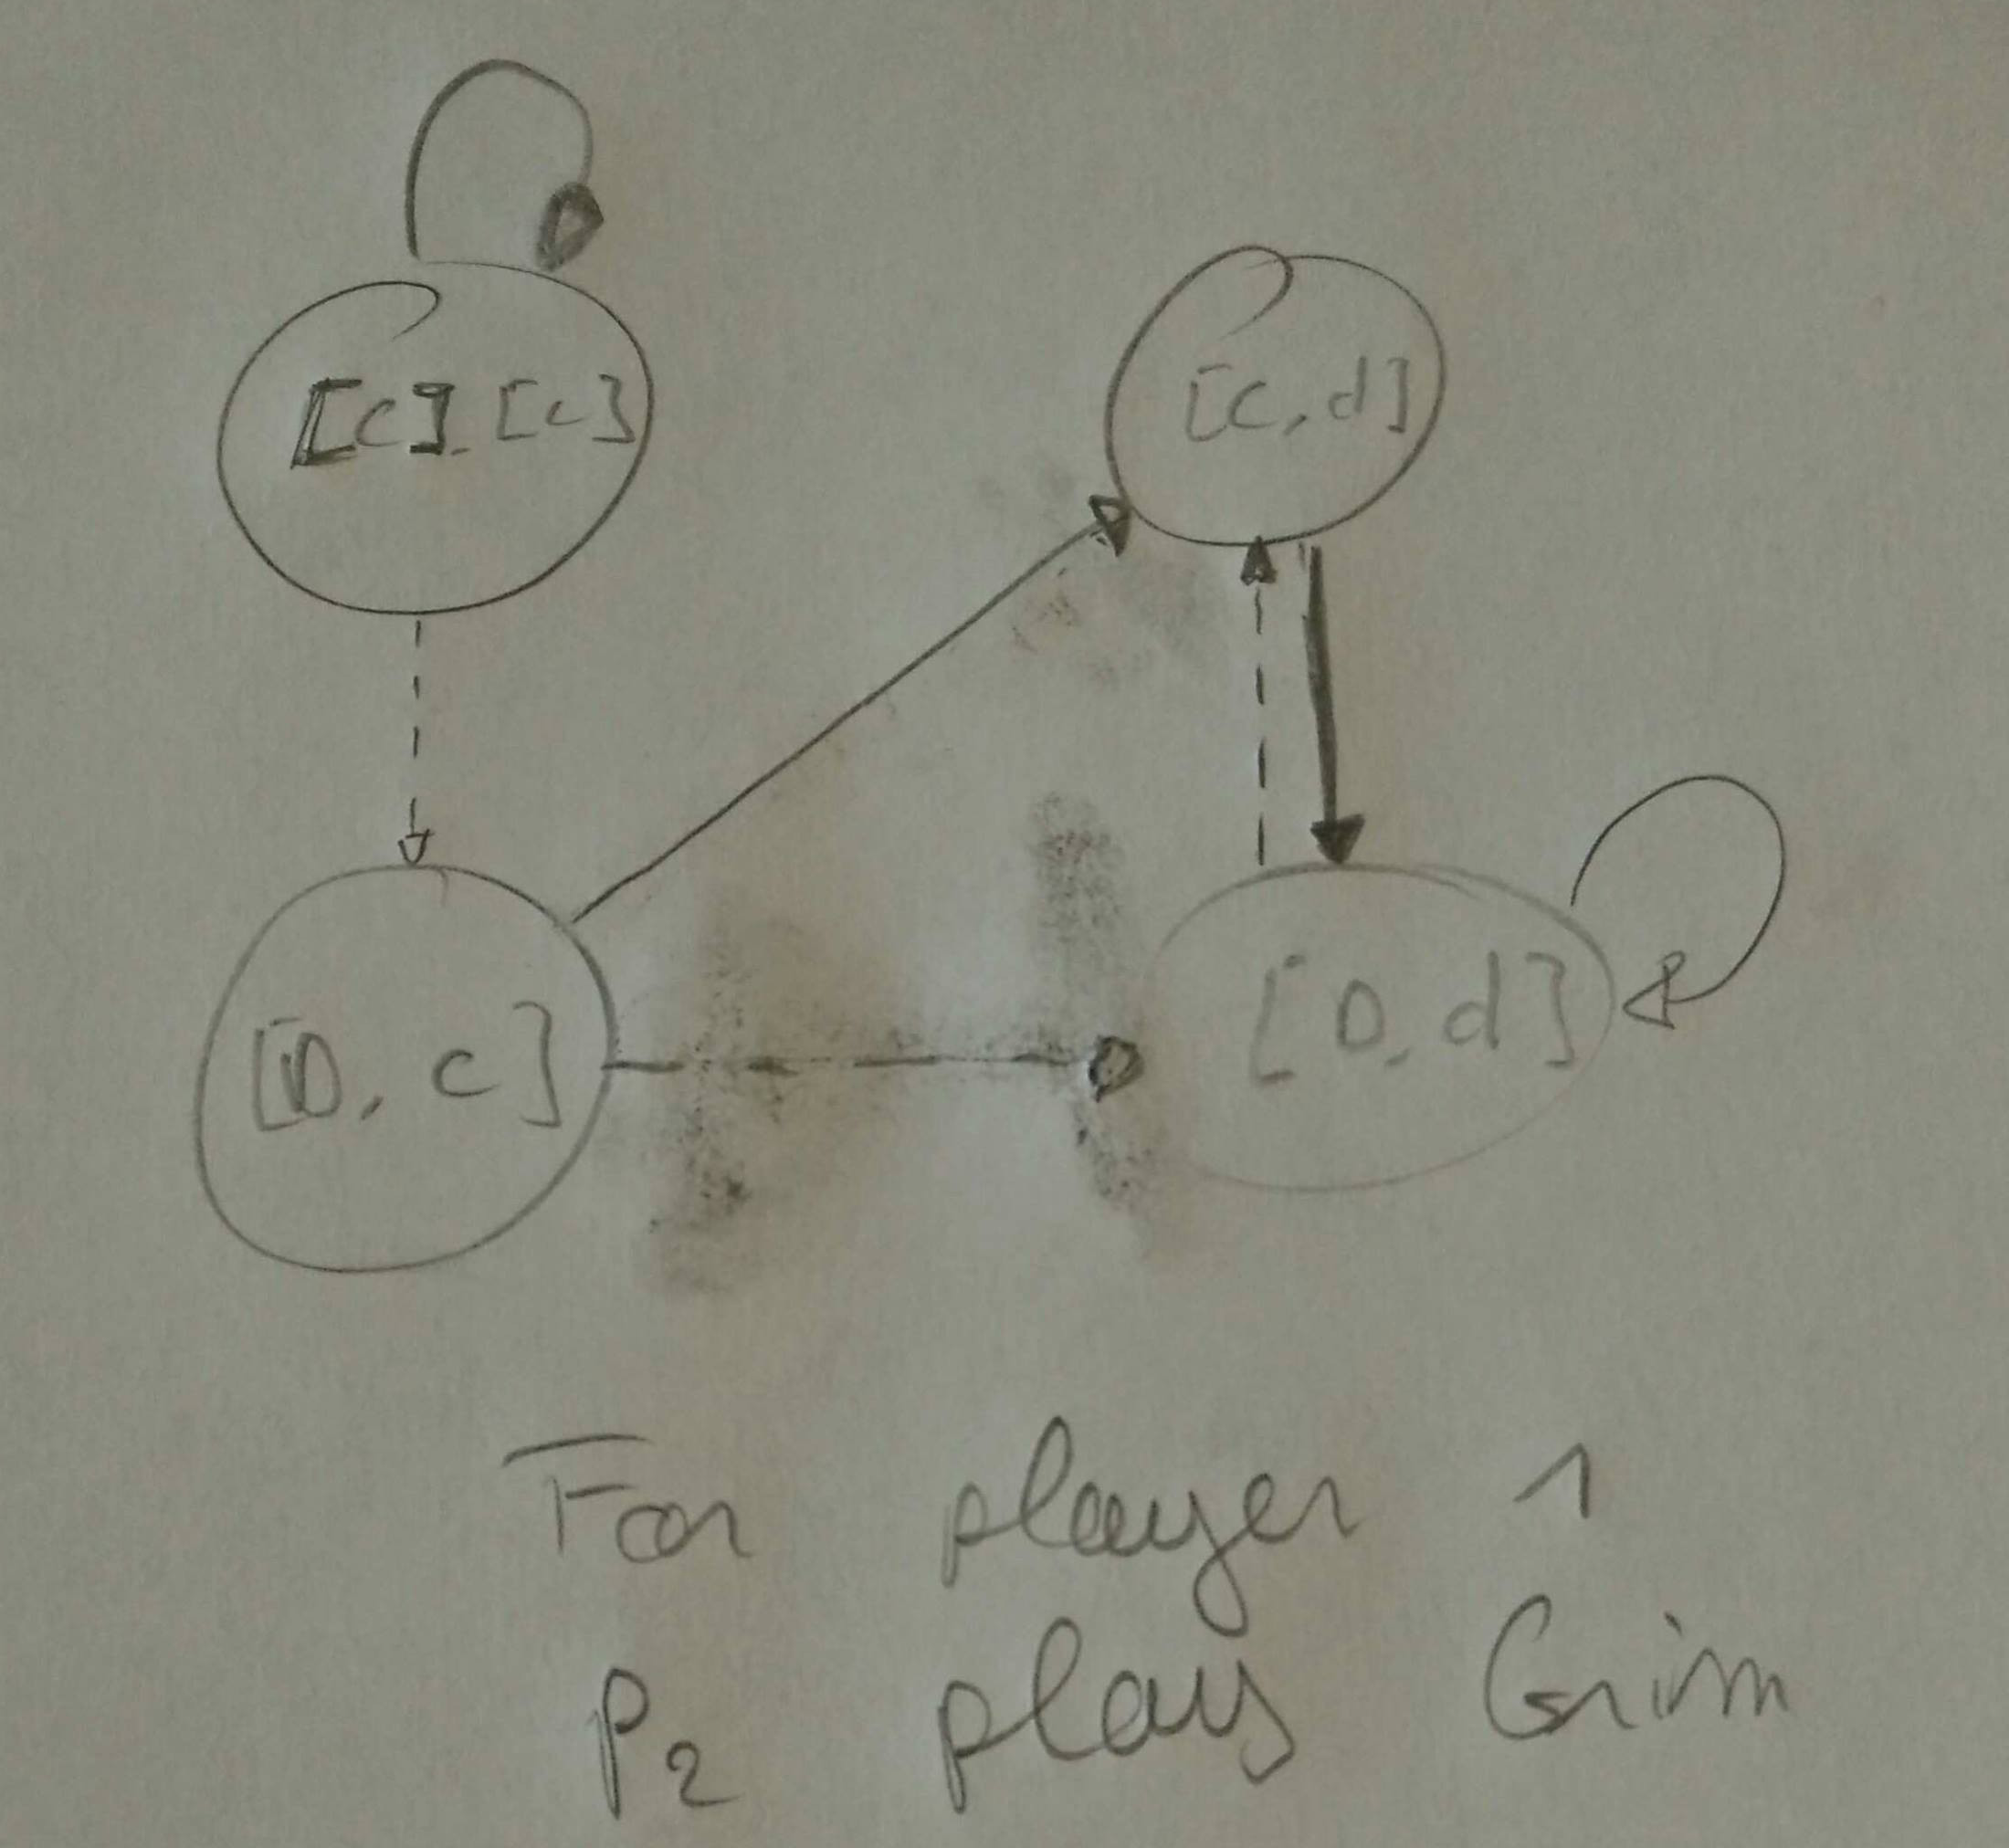
\includegraphics[width=0.5\linewidth]{img/ex_grim.jpg}	
	}
\end{minipage}

\end{frame}


\begin{frame}{Analyze the game}
Let's $\nu_i$ be the \textit{expected $\delta$-discounted average} of player $i$ when beginning from the state $\theta \in \Theta$ when everyone plays according to $\tau$.
\begin{small}
\begin{align*}
\nu_i(\theta, \tau) &=   \sum_{d_i \in D_i} \tau_i(d_i|\theta) \cdot Y_i(\tau, d_i, \nu_i, \theta, \delta)\\
&= \sum_{d_i \in D_i} \tau_i(d_i|\theta) \sum_{d_{-i} \in D_{-i}} \tau_{-i}(d_{-i} |\theta) \left( (1-\delta) u_i(d_i,\theta) + \delta \sum_{\hat{\theta}} p(\hat{\theta}|d,\theta) \nu_i(\hat{\theta},\tau) \right)  \\
&= \text{max}_{d_i \in D_i} Y_i(\tau, d_i, \nu_i, \theta, \delta)
\end{align*}
\end{small}
\begin{small}
\begin{align*}
Y_i(\tau, d_i, \nu_i, \theta, \delta) = \sum_{d_{-i} \in D_{-i}} \tau_{-i}(d_{-i} |\theta) \left( (1-\delta) u_i(d_i,\theta) + \delta \sum_{\hat{\theta}} p(\hat{\theta}|d,\theta) \nu_i(\hat{\theta},\tau) \right)
\end{align*}
\end{small}
This expression can be interpreted as the gain of player $i$ if he played the move $d_i$ once if at state $\theta$ everyone else follows $\tau$.
\end{frame}

\begin{frame}{Let's go back to the prisonner's dilema for a small example}
For a given $0 \leq \delta < 1$ we have the followin $\delta$-discounted payoff for player 1
	\begin{align*}
		\nu_1([C],[c]) &= (1-\delta) \cdot 1 + \delta \cdot \nu_1([C],[c])\\
		\nu_1([D],[c]) &= (1-\delta) \cdot -1 + \delta \cdot \nu_1([C],[c])\\
		\nu_1([C],[d]) &= (1-\delta) \cdot 2 + \delta \cdot \nu_1([C],[c])\\
		\nu_1([D],[d]) &= (1-\delta) \cdot 0 + \delta \cdot \nu_1([C],[c])
	\end{align*}
\pause
The solution are imediate:
\begin{align*}
	\nu_1([C],[c]) &= 1\\
	\nu_1([D],[c]) &= \frac{2\delta - 1}{1+\delta}\\
	\nu_1([C],[d]) &= \frac{2-\delta}{1+\delta}\\
	\nu_1([D],[d]) &= 0
\end{align*}
\end{frame}

\begin{frame}
	Then, to ensure that $\tau$ is an equilibrium of the repeated game, we must verify the equation $\nu_i(\theta) = \text{max}_{d_i \in D_i} Y_i(\tau, d_i, \nu_i, \theta, \delta)$. That is to ensure that the follwing inequalities are satisfied.
\begin{align*}
	\nu_1([C],[c]) &\geq (1-\delta)2 + \delta \nu_1([D],[c]) = \nu_1([C],[d]) \quad \text{Doing D instead of C}\\
	\nu_1([D],[c]) &\geq (1-\delta)0 + \delta \nu_1([D],[d]) = 0 \qquad \text{Doing D instead of C}\\
	\nu_1([C],[d]) &\geq (1-\delta)1 + \delta \nu_1([C],[c]) = 1 \qquad \text{Doing C instead of D}\\
	\nu_1([D],[d]) &\geq (1-\delta)(-1) + \delta \nu_1([C],[d]) = \nu_1([D],[c]) \quad \text{Doing C instead of D}
\end{align*}

\pause
\begin{itemize}
	\item For $\delta = 0.5$ : equilibrium reached
	\item For $\delta \leq 0.5$ : We play as for the non repetitive Prisoner's dilemma (search for immediate reward).
	\item For $\delta \geq 0.5$ : If we know that the other is going to play Tit-for-Tat, we should always play cooperate.
\end{itemize}
\end{frame}

\section{Standard Repeated Games}
\begin{frame}{Outline}
    \tableofcontents[currentsection]
\end{frame}

\begin{frame}{A Taxonomy of Repeated Games Models}
    \begin{figure}
        \tikzstyle{mybox} = [draw=gray!20, fill=white, very thick,
        rectangle, rounded corners, inner sep=10pt, inner ysep=10pt]
        \tikzstyle{fancytitle} = [fill=gray, text=white, rounded corners]
        \scalebox{0.7}{
        \begin{tikzpicture}
            \node [mybox] at (0, 0) (gen-mod){%
                \begin{minipage}{0.50\textwidth}
                    \vspace{-0.25cm}
                    \[ \Gamma^r = (N, \Theta, (D_i, S_i, u_i)_{i\in N}, q, p) \]
                \end{minipage}
            };
            \node [inner sep=0pt] (gen-mod-img) at (-4.4, 0.5){%
                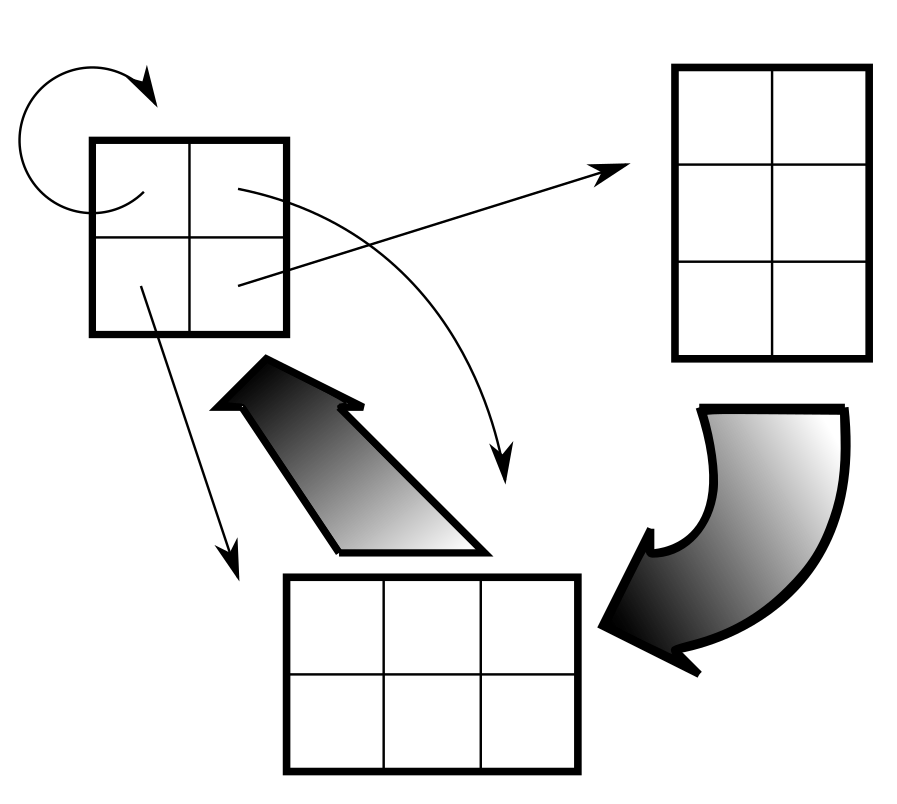
\includegraphics[width=0.25\textwidth]{img/stochastic.png}
            };
            
            \node [mybox] at (-4.5, -3) (mdp){%
                \begin{minipage}{0.40\textwidth}
                    {\color{green}Single-agent stochastic game}
                    \vspace{-0.25cm}
                    \[ |N| = 1. \]
                \end{minipage}
            };
            
            \node [mybox] at (0, -7.5) (state){%
                \begin{minipage}{\textwidth}
                    {\color{green}At every round, every player knows the
                    current state of nature $\theta \in \Theta$.} \\
                    Informally, for each player $i \in N$, there exists some
                    state $w(s_i) \in \Theta$ such that the signal $s_i$ can
                    never occur unless the current state is $w(s_i)$.
                \end{minipage}
            };
            
            \node [mybox, draw=black] at (4.5, -3.5) (std){%
                \begin{minipage}{0.60\textwidth}
                    \begin{itemize}
                        \item {\color{green}Only one possible state of
                        nature}
                        \[ |\Theta| = 1. \]
                        \item {\color{green}Players know all of each other's past
                        moves}
                        \[ S_i = \bigtimes_{j\in N-i} D_j. \]
                    \end{itemize}
                \end{minipage}
            };
            \node [inner sep=0pt] (gen-mod-img) at (7, -5.5){%
                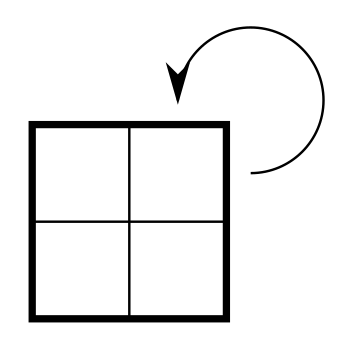
\includegraphics[width=0.20\textwidth]{img/std.png}
            };

            \node[fancytitle] at (gen-mod.north) {Stochastic Games (General Model)};
            \node[fancytitle] at (mdp.north) (mdp-title) {Markov Decision Processes};
            \node[fancytitle] at (state.north) (state-title) {Complete State Information};
            \node[fancytitle, fill=black] at (std.north) (std-title) {Standard Repeated Games};

            \draw[thick, -Latex] (gen-mod.west) -- (mdp-title.north);
            \draw[thick, -Latex] (gen-mod.south) -- (state-title.north);
            \draw[thick, -Latex] (gen-mod.east) -- (std-title.north);
        \end{tikzpicture}}
        \caption{A taxonomy of repeated game models.}
    \end{figure}
\end{frame}

\begin{frame}{Repeated game with standard information}
    \metroset{block=fill}
    \begin{block}{Definition}
        A \textbf{standard repeated game} is a repeated game in which there is only one state of
        possible state of nature
		$$|\Theta| = 1,$$
        the players know all of each other's past moves
        $$S_i = \bigtimes_{j \in N} D_j \quad \forall,$$
        and
		$$p(d,...,d,\theta | d, \theta) = 1 \quad \forall d \in D.$$
    \end{block}
\end{frame}


\begin{frame}{Example : the game of Chicken}
    \begin{exampleblock}{Example}
        Consider the game of Chicken in normal form
        \begin{table}
            \begin{tabular}{c|cc}
                & {\color{red}$a_2$}    & {\color{red}$b2$} \\
                \hline
                {\color{green}$a_1$}    & \payoff{4}{4}   & \payoff{1}{6} \\
                {\color{green}$b_1$}    & \payoff{6}{1}    & \payoff{-3}{-3} 
            \end{tabular}
            \caption{Game of Chicken in normal form}
        \end{table}
    
    \end{exampleblock}
    \note{
		Draw the normal form on the board    
		
		Explain the anecdote
    }
\end{frame}

\begin{frame}{Equilibrium of the single shot game}
\textbf{Analyze of the game}

\begin{itemize}
	\pause
	\item Nash equilibrium : (1,6) (6,1)
	\begin{itemize}
		\item Randomized equilibrium : $u_i = 0.5\cdot4 + 0.5 \cdot (6+1-3) = 3$
		\item Correlated equilibrium : $u_i = 0.5\cdot4 + 0.25 \cdot (6+1) =  3.75$
	\end{itemize}
	\pause
	\item Repetition of the game with standard information $$u_i = ??$$
\end{itemize}
	\pause
	Tit-for-tat is an equilibrium if $\delta \geq \frac{2}{3}$
\end{frame}

\note{
	Say that $(a_1,a_2)$ is not an sub-game perfect of the \textbf{one round} game because both players would want to play $b$

	\begin{itemize}
		\item \textbf{HYP}
			\begin{itemize}
				\item Infinitely repeated game with standard information
				\item Player 1 choose a $\delta$ between 0 and 1, what value of $\delta$
				\item Player 2 begin to be bold, and then be cautious at every round
			\end{itemize}
		\item Compute the $\delta$-discounted average payoff : $(1-\delta)(6+1\delta+\sum_{k=3}^\infty 4\delta^{k-1} ) = 6 - 5\delta + 3 \delta^2$
		\item $\delta$-discounted average if no deviation from tit-for-tat : $4 \geq 6 - 5\delta + 3 \delta^2$
		\item Tit-for-Tat is an equilibrium if $\delta \geq \frac{2}{3}$
	\end{itemize}
}

\begin{frame}{Going further with the Tit-for-Tat strategy in a standard information game}
	
	\textbf{Going further}
	\begin{itemize}
	\item What will be the $\delta$-discounted average payoff if both player decide to play Tit-for-Tat after player 2 deviation ?
	\pause
	
	\item What will be the $\delta$-discounted average payoff if p1 deviates from Tit-for-Tat after player 2 deviation. Then both play Tit-for-Tat.
	\pause
	\item What $\delta$ should we choose so that neither player can gain by being the first to deviate ?
	\end{itemize}
	\note{
	\textbf{Going further}
	\begin{itemize}
		\item If both player play Tit-for-tat after P2 deviation $(1-\delta)(1+6\delta+1\delta^2+6\delta^3+...) = \frac{1+6\delta}{1+\delta}$
		\item If P1 deviate after P2 deviation $(1-\delta)(1+4\delta+4\delta^2+4\delta^3+...) = 1+3\delta$
		\item $1+3\delta > \frac{1+6\delta}{1+\delta}$ when $\delta > \frac{2}{3}$
	\end{itemize}
	
	\textbf{Grim strategy}
	
	Only explain that such unforgiving punishment is not rational and extreme. We might be interested in finding other strategies.			
	}
\end{frame}

\begin{frame}{Finding mutual punishment strategies}
	\metroset{block=fill}
    \begin{block}{Mutual punishment strategy}
        For a player i, a {\color{green}mutual punishment strategy} can be :
        \begin{itemize}
        	\item On the first round : i plays $a_i$ \pause
        	\item If last round was $(a_1,a_2) \text{ or } (b_1,b_2)$, i plays $a_i$ \pause
        	\item If last round was $(a_1,b_2) \text{ or } (b_1,a_2)$, i plays $b_i$
        \end{itemize}
    \end{block}
    \textbf{\color{green}Interpretation}
    
    If both players follow the strategy, their expected payoff is 4. If one deviate, the other punish him until he participate himself in his own punishment.
    
    \textbf{\color{green}Is it a sub-game perfect equilibrium to follow the mutual punishment strategy?}
    
    \note{
		\textbf{If strategy call for $b_i$ but play $a_i$}
		
		Deviation is noob if $4+4\delta \geq 6 - 3 \delta \qquad \Rightarrow \delta \geq \frac{2}{7}$ not worth to deviate
		
		\textbf{If strategy call for $a_i$ but play $b_i$}
		
		Deviation is noob if $-3+4\delta \geq 1 - 3\delta \qquad \Rightarrow \delta	\geq \frac{4}{7}$ not worth to deviate
		
		    
    }
\end{frame}

\begin{frame}{Take home message \#6}
    \metroset{block=fill}

    \begin{block}{Take-home-message \#6}
        \vspace{0.2cm}
        \begin{columns}
            \begin{column}{0.65\textwidth}
                A \textbf{repeated game with standard information} is a repeated game where
                \begin{itemize}
                    \item there is {\color{green}only one possible state of nature}
                    \item the players {\color{green}know all of each other's past moves}
                \end{itemize}
            \end{column}
            \begin{column}{0.2\textwidth}
                \begin{center}
                    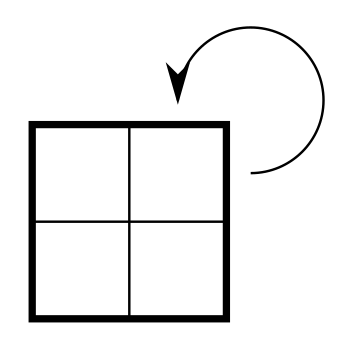
\includegraphics[width=0.7\linewidth]{img/std.png}
                \end{center}
            \end{column}
        \end{columns}

        \vspace{0.5cm}
        Depending on the value of the discount factor $\delta$, several strategies might constitute
        an equilibrium: \textit{tit-for-tat}, \textit{getting-even}, \textit{grim}, etc.
        However, these equilibria might not always be subgame perfect.
    \end{block}
\end{frame}


\section{Folk Theorem}
\begin{frame}{Outline}
    \tableofcontents[currentsection]
\end{frame}


\begin{frame}{Folk Theorem}
    \textbf{Strategy in infinitely-repeated game}\\
    \begin{itemize}
        \item Choice of action at every decision point
        \item No finite set of pure strategies!
        \item Nash theorem doesn't apply anymore\\
        $\rightarrow$ We need new rules
    \end{itemize}
\end{frame}



\begin{frame}{Enforceability and feasability}
    \begin{itemize}
        \item Consider any $n$-player game $\Gamma = (N, D, u)$ and any payoff vector
        $u = (u_1, \dots, u_n)$.
        \item Let $v_i= \min_{d_{-i}\in D_{-i}} \max_{d_i\in D_i} u_i(d_{-i}, d_i)$ be
        the minmax value of player $i$.
    \end{itemize}
    \metroset{block=fill}

    \begin{block}{Enforceable payoff profile}
        A payoff profile $u$ is \textbf{enforceable} if $u_i \geq v_i$.
    \end{block}

    \begin{block}{Feasible payoff profile}
        A payoff profile $u$ is \textbf{feasible} if there exist rational, non-negative
        values $\alpha_d$ such that for all $i$, we can express $u_i$ as
        $\sum_{d\in D} \alpha_d u_i(d)$, with $\sum_{d\in D} \alpha_d = 1$.
    \end{block}
\end{frame}

\begin{frame}{Folk Theorem with average rewards}
    \metroset{block=fill}

    \begin{block}{The Folk theorem with average rewards}
        Consider any $n$-player normal-form game $\Gamma$ and any payoff profile
        $u = (u_1, \dots, u_n)$. Then\footnote{This version of the theorem is proven
        in the book "\textbf{Multiagent Systems}, Algorithmic, Game-Theoretic, and Logical
        Foundations".}
        \begin{enumerate}
            \item If $u$ is the payoff profile in any Nash equilibrium of the infinitely
            repeated $\Gamma$ with average rewards, then for each player $i$, $u_i$ is enforceable.
            \item If $u$ is both feasible and enforceable, then $u$ is the payoff profile for some
            Nash equilibrium of the infinitely repeated $\Gamma$ with average rewards.
        \end{enumerate}
    \end{block}
\end{frame}
\note{
    \begin{block}{Folk Theorems}
        \begin{itemize}
            \item Theorems that circulate among mathematicians but cannot be traced back to one individual
            \item Considered to have established status but generally no proof in complete form
            \item One notable one in Game Theory, that we are going to see today
        \end{itemize}
    \end{block}
}


\begin{frame}{Interpretation of the Folk theorem}
    \begin{exampleblock}{What does it mean?}
        \begin{itemize}
            \item The first part of the theorem means that we can enforce any Nash equilibrium
            of the infinitely-repeated game
            \item The second part states that any payoff profile that is feasible and enforceable
            is the payoff profile of a Nash equilibrium 
        \end{itemize}
    \end{exampleblock}
\end{frame}

\begin{frame}{Folk Theorem}
    \textbf{Consequences}\\
    \begin{itemize}
        \item Interesting consequences: apparition of new Nash equilibrium's for certain games
        \item Example: prisoner's dilemna
        \begin{itemize}
            \item If game goes on long enough (proba of 1 more turn $\rightarrow 1$), cooperation of both
            players becomes a Nash equilibrium
        \end{itemize}
    \end{itemize}
\end{frame}

\begin{frame}{Folk Theorem}
    \begin{exampleblock}{Example}
        Consider the Prisoner's Dilemma in normal form.
        \begin{table}
            \begin{tabular}{c|cc}
                & {\color{red}c}    & {\color{red}d} \\
                \hline
                {\color{green}C}    & \payoff{-1}{-1}   & \payoff{-4}{~0} \\
                {\color{green}D}    & \payoff{~0}{-4}    & \payoff{-3}{-3} 
            \end{tabular}
            \caption{Prisoner's Dilemma in normal form.}
        \end{table}
    \end{exampleblock}
\end{frame}

\note{
    Simply prove that cooperation is feasible and enforceable:\\
    \begin{itemize}
        \item Enforceability
            $v_1=\min_{s_{-1}\in S_{-1}} \max_{s_{1}\in S_{1}} u_1(s_{-1},s_1) =-3$\\
            $v_2=\min_{s_{-2}\in S_{-2}} \max_{s_{2}\in S_{2}} u_2(s_{-2},s_2) =-3$\\
            $r_1=1\geq -3$,$r_2=1\geq -3 \rightarrow$ enforceable \\
        \item Feasibility
            $\alpha_{(c,C)}= 1$, rest $\alpha=0 \rightarrow$ feasible
    \end{itemize}
    By Folk theorem $\rightarrow$ Nash equilibrium
}

\begin{frame}{Take-home message \#7}
    \metroset{block=fill}
    \begin{block}{Take-home message \#7}
        By the \textbf{Folk theorem} with average rewards
        \begin{center}    
            payoff Nash equilibrium $\leftrightarrow$ payoff feasible and enforceable.
        \end{center}
    \end{block}
\end{frame}


\section{Learning Rules}
\begin{frame}{Outline}
    \tableofcontents[currentsection]
\end{frame}


\begin{frame}{Learning rules}
    \textbf{Definition}
    \begin{itemize}
        \item Learning strategy: Use of previous information to improve its behavior
        \item Deeply linked with artificial intelligence
    \end{itemize}
\end{frame}

\begin{frame}{Learning rules}
    \textbf{Two types of theories}
    \begin{itemize}
        \item Descriptive theories: theories that attempt to study the way learning takes place in real life
        \item Prescriptive theories: theories that study the way agents \textit{should} react in real life
    \end{itemize}
\end{frame}

\begin{frame}{Descriptive theories}
    \textbf{Properties}
    \begin{itemize}
        \item \textbf{Realism}: There should be a good match between the formal theory and the natural phenomenon being studied
        \item \textbf{Convergence}: The theory should exhibit convergence of the strategy profile to some equilibrium
    \end{itemize}
\end{frame}

\begin{frame}{Prescriptive theories}
    \textbf{Properties}
    \begin{itemize}
        \item \textbf{Safety}: Guarantees the agent at least learning rule its maxmin payoff, or “security value.”
        \item \textbf{Rationality}: Whenever the opponent's learning rule settles on a stationary strategy the agent settles on a best response to that strategy
        \item \textbf{No-regret}: Yields a better result that any pure strategy the agent could have played
    \end{itemize}
\end{frame}

\begin{frame}{Fictitious play}
    \textbf{Fictitious play}
    \begin{itemize}
        \item One of the earliest learning rules 
        \item Instance of model-based learning where learner maintains belief about opponent
        \item Agent believes that his opponent is playing the mixed strategy given by the empirical distribution of the opponent’s previous actions
    \end{itemize}
\end{frame}

\begin{frame}{Fictitious play}
    \begin{algorithm}[H]
         Initialize beliefs about the opponent strategy\;
         \While{true}{
            Play a best response to the assessed strategy of the opponent\\
            Observe the opponent’s actual play and update beliefs accordingly\\
         }
    \caption{Fictitious play algorithm}
    \end{algorithm}
\end{frame}


\begin{frame}{No-regret playing}
    \textbf{Regret}\\
    \textit{Let $\alpha^t$ be the average per-period reward the agent received up to time $t$ and $\alpha^t(s)$ the average per-period reward the agent would have received by playing strategy $s$.}\\
    \textit{The regret an agent experiences at time $t$ for not having played $s$ is $R^t(s)=\alpha^t-\alpha^t(s)$}
\end{frame}

\begin{frame}{No-regret playing}
    \textbf{No-regret learning rule}\\
    \textit{A learning rule exhibits \textbf{no regret} if it guarantees with high probability that the agent will not experience any positive regret}
\end{frame}

\begin{frame}{No-regret playing}
    \textbf{Example of a no-regret strategy: Regret matching}\\
    \begin{itemize}
        \item At each time step each action is chosen with probability consistent to its regret
        \item The strategy of playing strategy $s$ at timestep $t+1$ is equal to:
        \[
            \sigma_i^{t+1}(s)= \frac{R^t(s)}{\sum_{s'\in S_i} R^t(s')}
        \]
    \end{itemize}
\end{frame}


\section{Game Theory in Communications: Power Control}
\begin{frame}{Outline}
    \tableofcontents[currentsection]
\end{frame}

\usetikzlibrary{calc}
\usetikzlibrary{decorations.pathreplacing,decorations.markings,shapes.geometric}
\tikzset{naming/.style={align=center,font=\small}}
\tikzset{antenna/.style={insert path={-- coordinate (ant#1) ++(0,0.25) -- +(135:0.25) + (0,0) -- +(45:0.25)}}}
\tikzset{station/.style={naming,draw,shape=dart,shape border rotate=90, minimum width=10mm,
minimum height=10mm,outer sep=0pt,inner sep=3pt}}
\tikzset{mobile/.style={naming,draw,shape=rectangle,minimum width=12mm,minimum height=6mm, outer sep=0pt,
inner sep=3pt}}
\tikzset{radiation/.style={{decorate,decoration={expanding waves,angle=90,segment length=4pt}}}}
\tikzset{middlearrow/.style 2 args={decoration={markings,mark=at position 0.5 with {\node[#1] {#2};}},
postaction={decorate}}}

\newcommand{\BS}[1]{%
	\begin{tikzpicture}
		\node[station] (base) {#1};
		\draw[line join=bevel] (base.100) -- (base.80) -- (base.110) -- (base.70) -- (base.north west)
        -- (base.north east);
		\draw[line join=bevel] (base.100) -- (base.70) (base.110) -- (base.north east);
		\draw[line cap=rect] ([yshift=0pt]base.north) [antenna=1];
	\end{tikzpicture}
}

\newcommand{\UE}[1]{%
	\begin{tikzpicture}
        \node (ue) {$\underset{#1}{\smartphone}$};
	\end{tikzpicture}
}

\begin{frame}{The need for Game Theory in communication systems}
    \begin{itemize}
        \item \textbf{There is a vast litterature on using game theory in communications.}
        \item Agents could be \textit{user equipments} (e.g. smartphones, tablets),
        \textit{base stations} (e.g. in 4G), \textit{mobile operators} (Orange, Proximus), etc.
    \end{itemize}

    \pause
    \begin{alertblock}{But the behaviour of each agent is supposed to be compliant with strict
    technical standards. Why do we need game theory here?}
        \begin{itemize}
            \pause
            \item Manufacturers may have incentives to develop products which behave selfishly
            to obtain a performance advantage over other network users ;
            \pause
            \item End users may have the capability to alter products to behave in a selfish
            manner.
        \end{itemize}
    \end{alertblock}

    \pause
    $\to$ We cannot simply rely on standards. {\color{green}Systems should be designed to
    make selfish behaviors unprofitable.}
\end{frame}

\begin{frame}{An interesting though on Game Theory}
    In~\cite{mackenzie01}, MacKenzie and Wicker argue

    \begin{center}
        ``\textit{In some sense, game theory is better suited to solving communications
        problem -- where the agents are likely to be computers -- than to solving economic
        problems.}''
    \end{center}
    
    \vspace{0.5cm}
    \textbf{{\color{green}The strong rationality assumption underlying game theory is more
    reasonnable for machines than human beings.}}
\end{frame}

\note{
    At this point, make the parallel with~\cite{pd-repeated-real-life} and potentially with
    the result of the first game played by the audience.
}

\begin{frame}{Problem description: players and strategy space}
    \begin{exampleblock}{Players and strategy space}
        \begin{itemize}
            \pause
            \item Players are smartphones willing to upload some data to a single base station (e.g. in
            a 4G network)
            \pause
            \item The power attenuation between player $i$ and the base station is $h_i \ge 0$
            \pause
            \item Each player controls its transmitted power level $p_i \ge 0$
        \end{itemize}
    \end{exampleblock}
\end{frame}

\begin{frame}{Problem description: illustration}
    \begin{figure}
        \centering
        \begin{tikzpicture}
            \node at (0, 0) (BS) {\BS{BS}};
            \node at (-2, 1) (UE1) {\UE{1}};
            \node at (-2, -1) (UE2) {\UE{2}};
            \node at (0, -2.5) (UE3) {\UE{3}};
            \node at (2, 1) (UE4) {\UE{5}};
            \node at (2, -1) (UE5) {\UE{4}};

            \draw[middlearrow={above}{$h_1$}, -Latex] (UE1) --  (BS);
            \draw[middlearrow={above}{$h_2$}, -Latex] (UE2) -- (BS);
            \draw[middlearrow={left}{$h_3$}, -Latex] (UE3) -- (BS);
            \draw[middlearrow={above}{$h_5$}, -Latex] (UE4) -- (BS);
            \draw[middlearrow={above}{$h_4$}, -Latex] (UE5) -- (BS);
        \end{tikzpicture}
        \caption{A simplified view of the uplink channels in a cellular network.}
    \end{figure}
\end{frame}

\begin{frame}{Problem description: utility (1)}
    \begin{exampleblock}{Utility: what does each player want?}
        \begin{itemize}
            \item Each player $i$ wants to increase
            \[ \text{SINR}_i = \frac{h_ip_i}{\sum_{j\neq i} h_jp_j 
                + \underbrace{\sigma^2}_\text{noise power}} \]
            This corresponds to \textbf{decreasing their interference level} at the base station.
            \item Each player $i$ wants to avoid using too much power $p_i$. This corresponds
            to \textbf{saving their battery life}.
        \end{itemize}
    \end{exampleblock}

    \vspace{0.5cm}
    $\to$ Units: (number of successfully transmitted bit) per (Joule used).
\end{frame}

\begin{frame}{Problem description: utility (2)}
    \begin{figure}
        \centering
        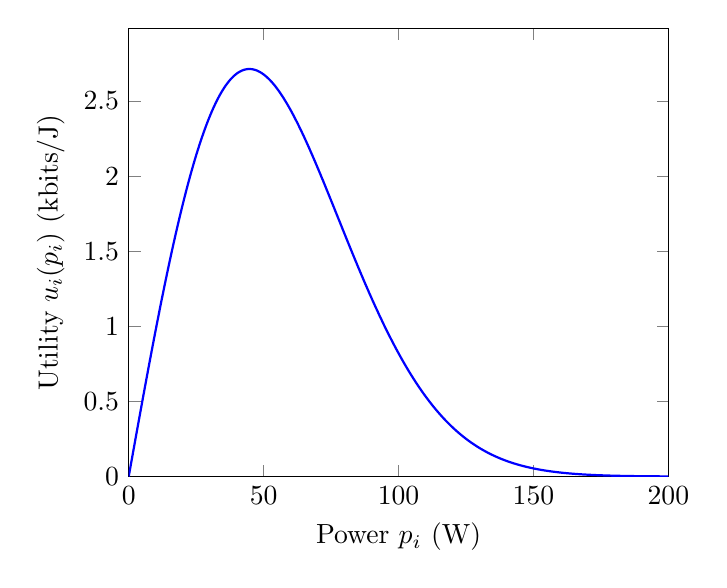
\begin{tikzpicture}
            \begin{axis}[
                    ylabel = {Utility $u_i(p_i)$ (kbits/J)},
                    xlabel = {Power $p_i$ (W)},
                    domain = 0:200,
                    samples = 1000,
                    xmin = 0,
                    xmax = 200,
                    ymin = 0
                ]
                \addplot[
                    color = blue,
                    thick
                ]
                {(x/10)*exp(-x^2/(2*2000))};
            \end{axis}
        \end{tikzpicture}
        \caption{Example of an utility function for a player}
    \end{figure}
\end{frame}

\note{
    Intuition behind this utility function:
    \begin{itemize}
        \item If $p_i$ is too low, the signal from player $i$ suffers too much from interference
        and is not well received by the base station.
        \item If $p_i$ is too high, the battery level of player $i$ is decreasing too quickly.
    \end{itemize}
}

\begin{frame}{The single-shot game}
    \begin{block}{Where is the game here?}
        Increasing $\text{SNR}_i$ requires increasing $p_i$, this will decrease $\text{SINR}_j$ and
        thus decrease other players utility.
    \end{block}
    \pause 
    \vspace{0.5cm}
    \begin{alertblock}{The Nash Equilibrium of the single-shot game is Pareto inefficient}
        In the same way the Nash Equilibirum of the single-shot Prisoner's Dilemma is
        Pareto inefficient...
    \end{alertblock}
    \pause
    \vspace{0.5cm}
    \textbf{{\color{green}Can we do better in a repeated game settings to force a better outcome?}}
\end{frame}

\begin{frame}{The repeated game model}
    \begin{exampleblock}{The repeated game model}
        \begin{itemize}
            \pause
            \item \textbf{Rounds}: a round corresponds to a packet transmission.
            \pause
            \item \textbf{Criterion for ranking payoffs}: we use the $\delta$-discounted average with a
            discount factor $\delta$ very close to 1 (can you guess why?).
            \pause
            \item \textbf{Signals}: after each transmitted packet, the base station informs each player
            of the received power level of each user.
            \pause
            \item \textbf{State of nature}: two possible cases
            \begin{enumerate}
                \pause
                \item the power attenuations $h_i$ are constant: only one state\\
                $\to$ standard repeated game,
                \pause
                \item the power attenuations $h_i$ vary in time: multiple states\\
                $\to$ stochastic game.
            \end{enumerate}
        \end{itemize}
    \end{exampleblock}
\end{frame}

\note{
    $\delta$ is very close to 1 because the time slot for the transmission of a single packet
    is typically very short (on the order of a few tens of microseconds).
}

\begin{frame}{Equilibrium strategy}
    \begin{block}{Equilibrium strategy}
        \begin{itemize}
            \item As long as no users exceeds the received power level, the system operates normally ;
            \item If a player behaves selfishly, all the other players transmit at maximum power level
            during the next time slot as a punishment.
        \end{itemize}
    \end{block}

    \vspace{0.5cm}
    \textbf{{\color{green}This strategy forms a new equilibrium more Pareto efficient than the
    single-shot Nash equilibrium.}}
\end{frame}


\begin{frame}{References}
    \nocite{*}
    \bibliographystyle{plain}
    \bibliography{biblio}
\end{frame}

\begin{frame}[standout]
    Questions?
\end{frame}

\end{document}
